\documentclass[11pt]{beamer}
\usetheme{Szeged}
\usepackage[utf8]{inputenc}
\usepackage{amsmath}
\usepackage{amsfonts}
\usepackage{amssymb}
\usecolortheme{dolphin}
\author{Kyle Colton\\Thomas Kwak}
\title{Classification of Land Types Through Clustering}
%\setbeamercovered{transparent} 
%\setbeamertemplate{navigation symbols}{} 
%\logo{}
\usepackage{animate}
\institute{Math 191} 
\date{\today}
\subject{Indian Pines Hyperspectral Imaging}
\begin{document}

\begin{frame}
\titlepage
\end{frame}

%%%%%%%%%%%%%%%%%%%%%%%%
%%%   Introduction   %%%
%%%%%%%%%%%%%%%%%%%%%%%%

\section{Introduction}
\subsection{Problem}
\begin{frame}{Data Set}
The \texttt{indian\_pines} dataset consists of hyperspectral earth images of farmland
\begin{columns}[T]
\begin{column}{.48\textwidth}
% LEFT COLUMN
\begin{itemize}
\item Dimensions $145 x 145 x 200$
\item Each image is $145x145$
\end{itemize}
\end{column}
\hfill
\begin{column}{.48\textwidth}
% RIGHT COLUMN
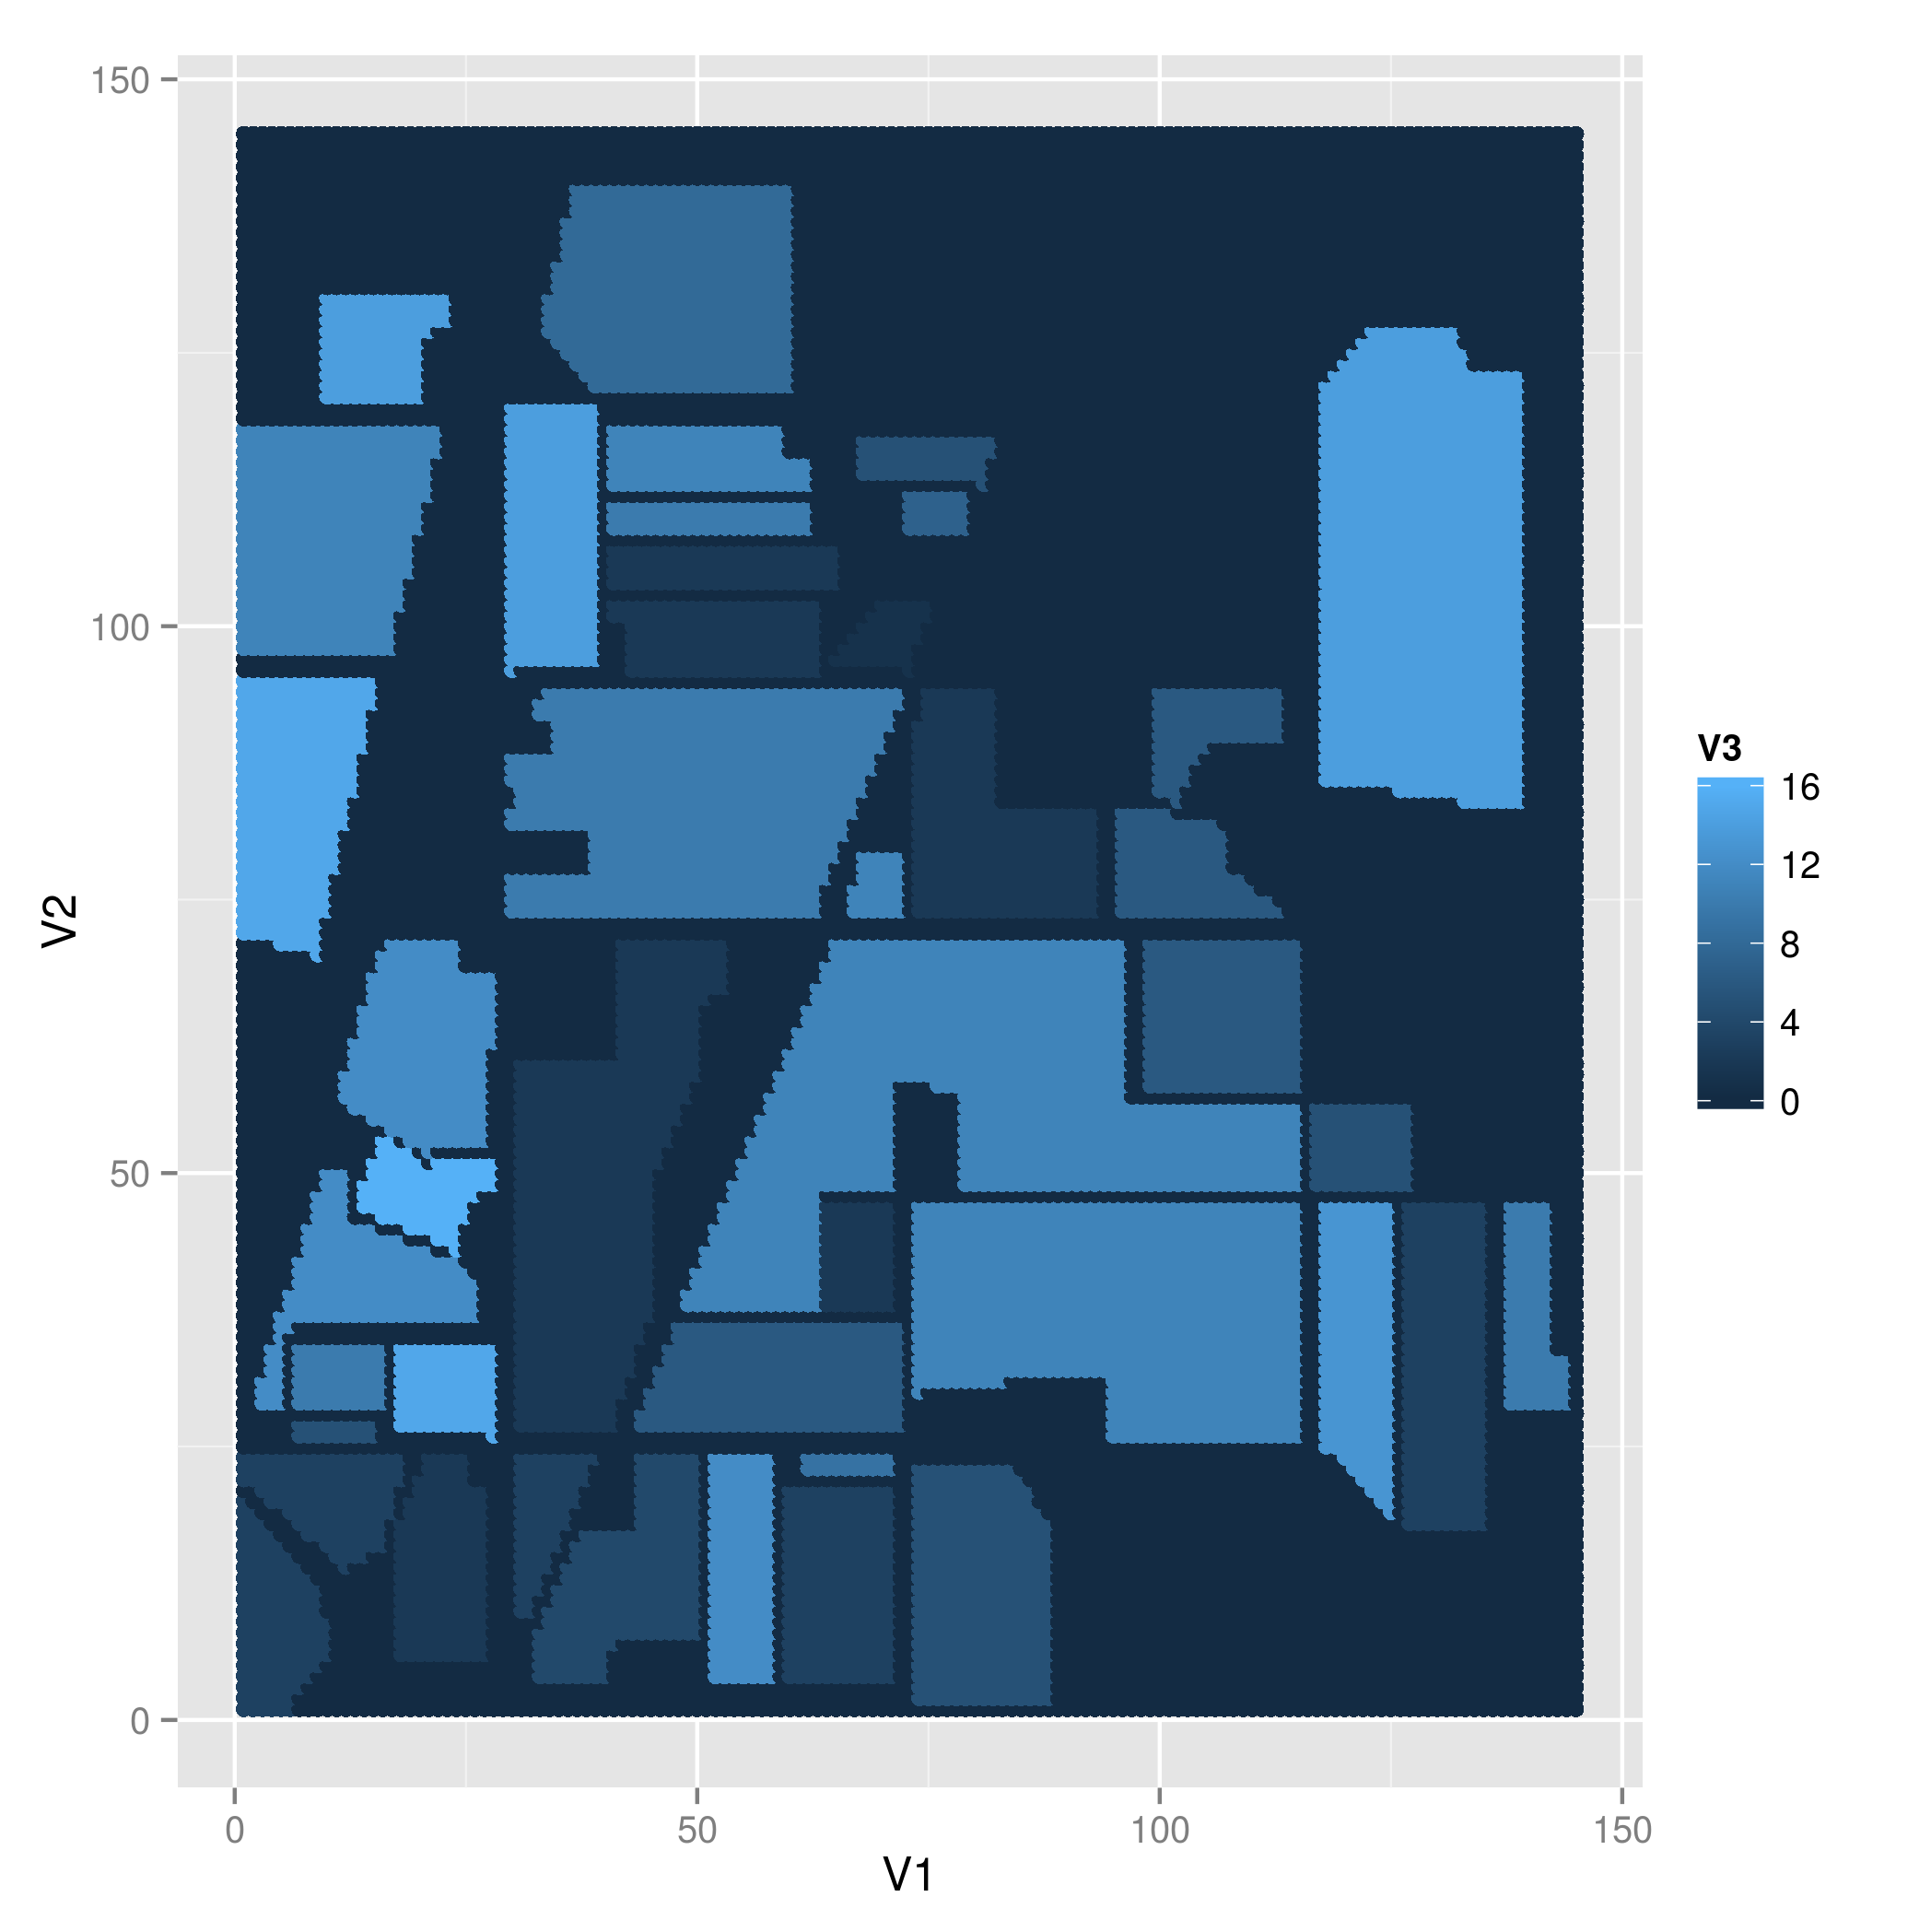
\includegraphics[scale=.3]{gt.png}
\end{column}
\end{columns}
\end{frame}

\begin{frame}{Data Set}
The \texttt{indian\_pines} dataset consists of hyperspectral earth images of farmland
\begin{columns}[T]
\begin{column}{.48\textwidth}
% LEFT COLUMN
\begin{itemize}
\item Images were captured at 200 different wavelengths
\item A total of 16 crops were used in the data set
\end{itemize}
\end{column}
\hfill
\begin{column}{.48\textwidth}
% RIGHT COLUMN
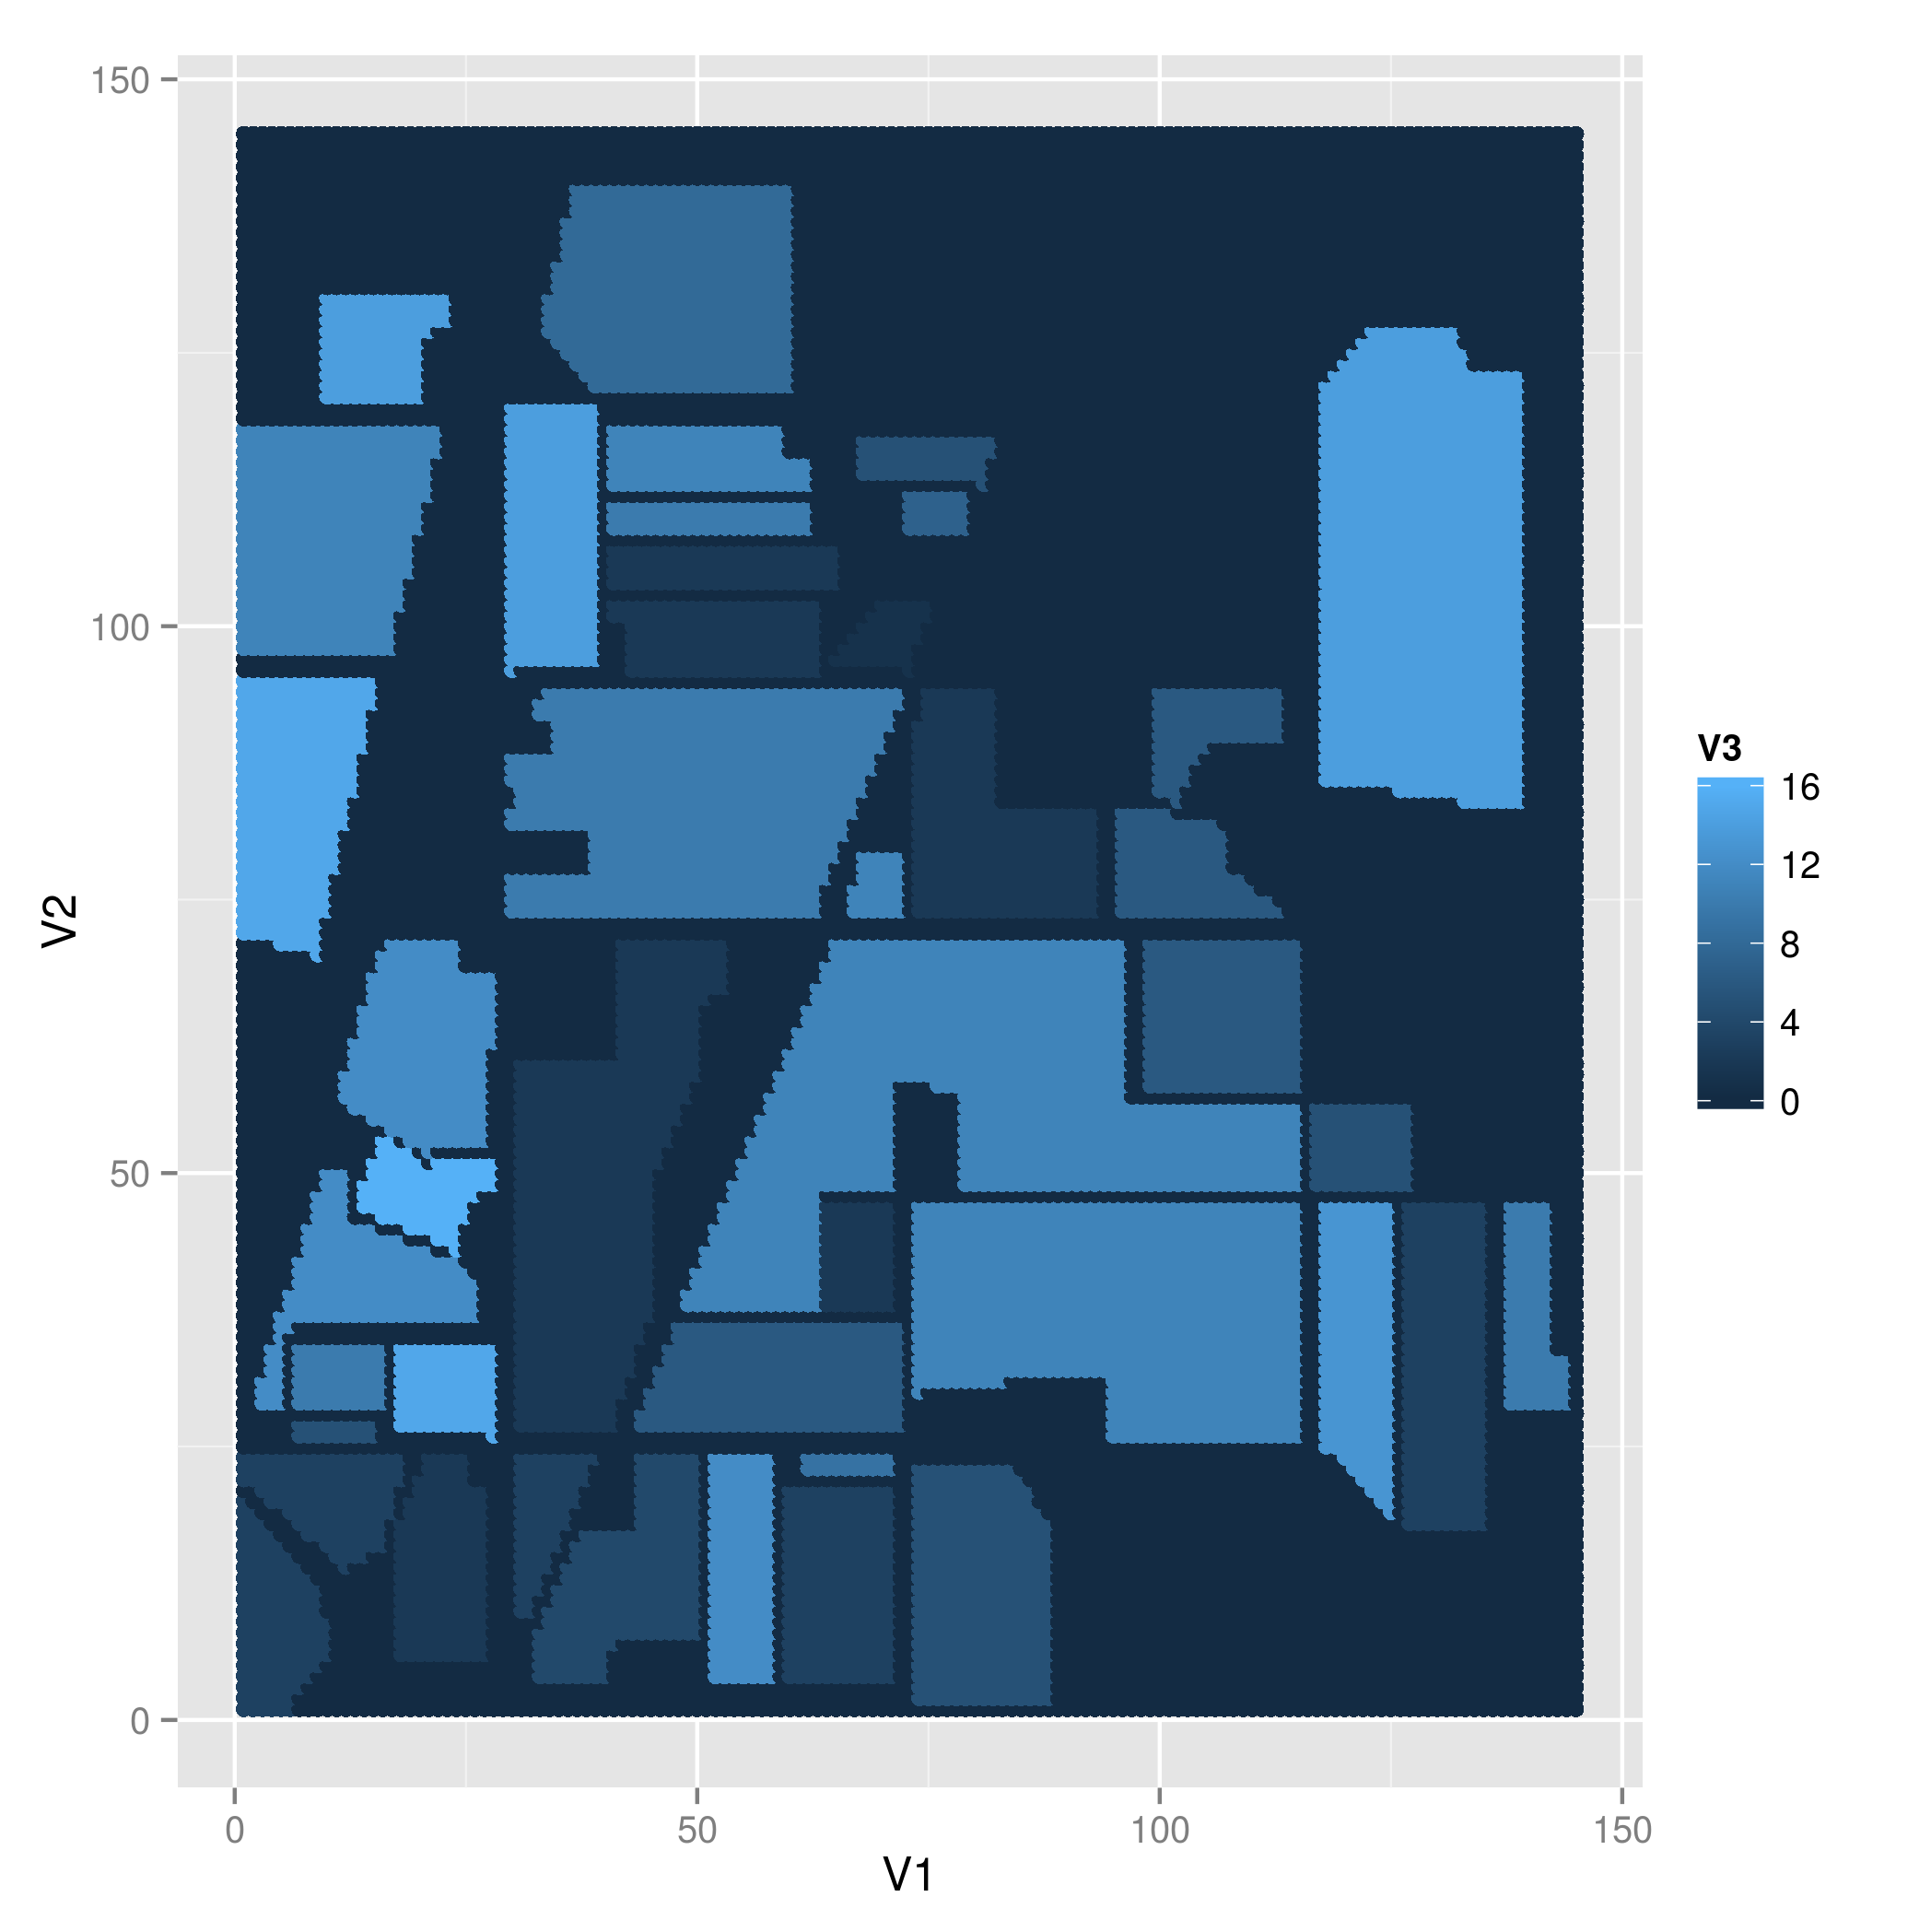
\includegraphics[scale=.3]{gt.png}
\end{column}
\end{columns}
\end{frame}

\subsection{Exploration}
\begin{frame}{Exploring the Data}
\begin{center}
% To run this, you must first convert the GIF to a series of PNGs
% bash: convert indian_pines.gif indian_pines_%d.png
\animategraphics[autoplay,loop,height=6cm]{10}{indian_pines_}{0}{199}
\end{center}
\end{frame}

\begin{frame}{Historgrams}
\begin{center}
% To run this, you must first convert the GIF to a series of PNGs
% bash: convert histograms.gif histograms_%d.png
\animategraphics[autoplay,loop,height=6cm]{10}{histograms_}{0}{199}
\end{center}
\end{frame}

%%%%%%%%%%%%%%%%%%%
%%%   K-Means   %%%
%%%%%%%%%%%%%%%%%%%

\section{K-Means}
\subsection{Lower order K-Means}
\begin{frame}{K-Means}
K-Means using 2 classes
\begin{columns}[T]
\begin{column}{.48\textwidth}
% LEFT COLUMN
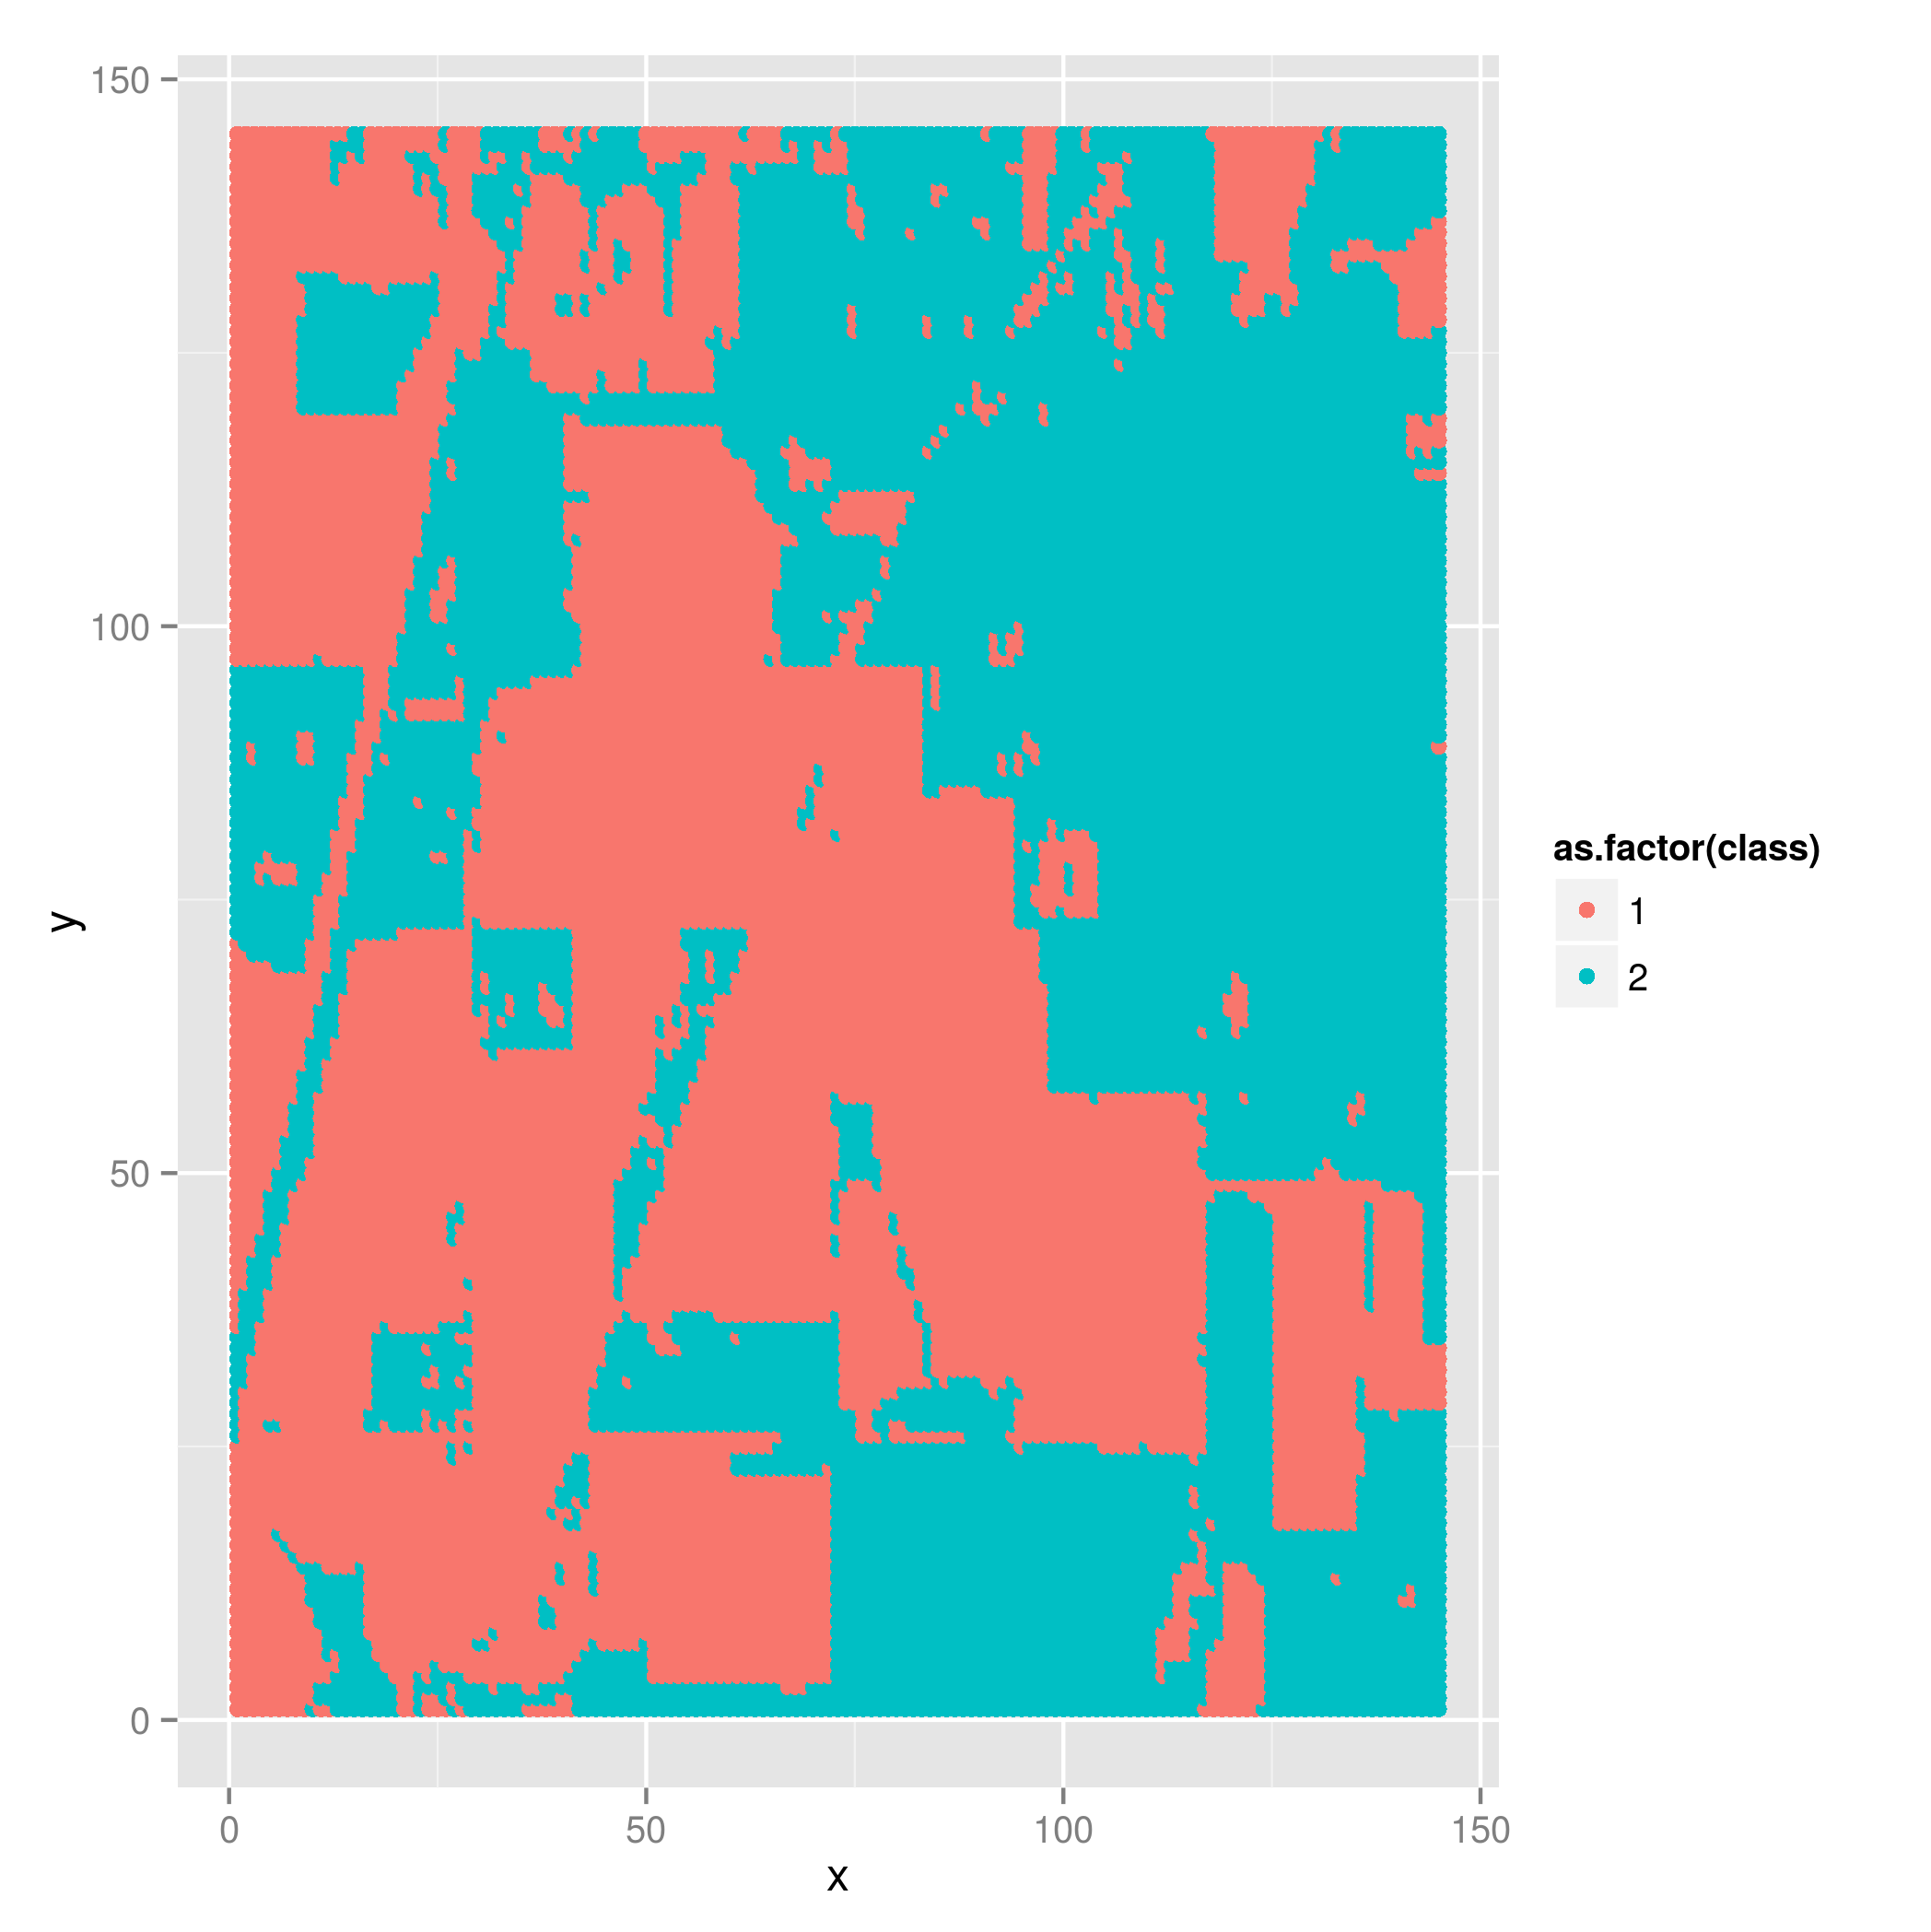
\includegraphics[scale=.3]{km2.png}
\end{column}
\hfill
\begin{column}{.48\textwidth}
% RIGHT COLUMN
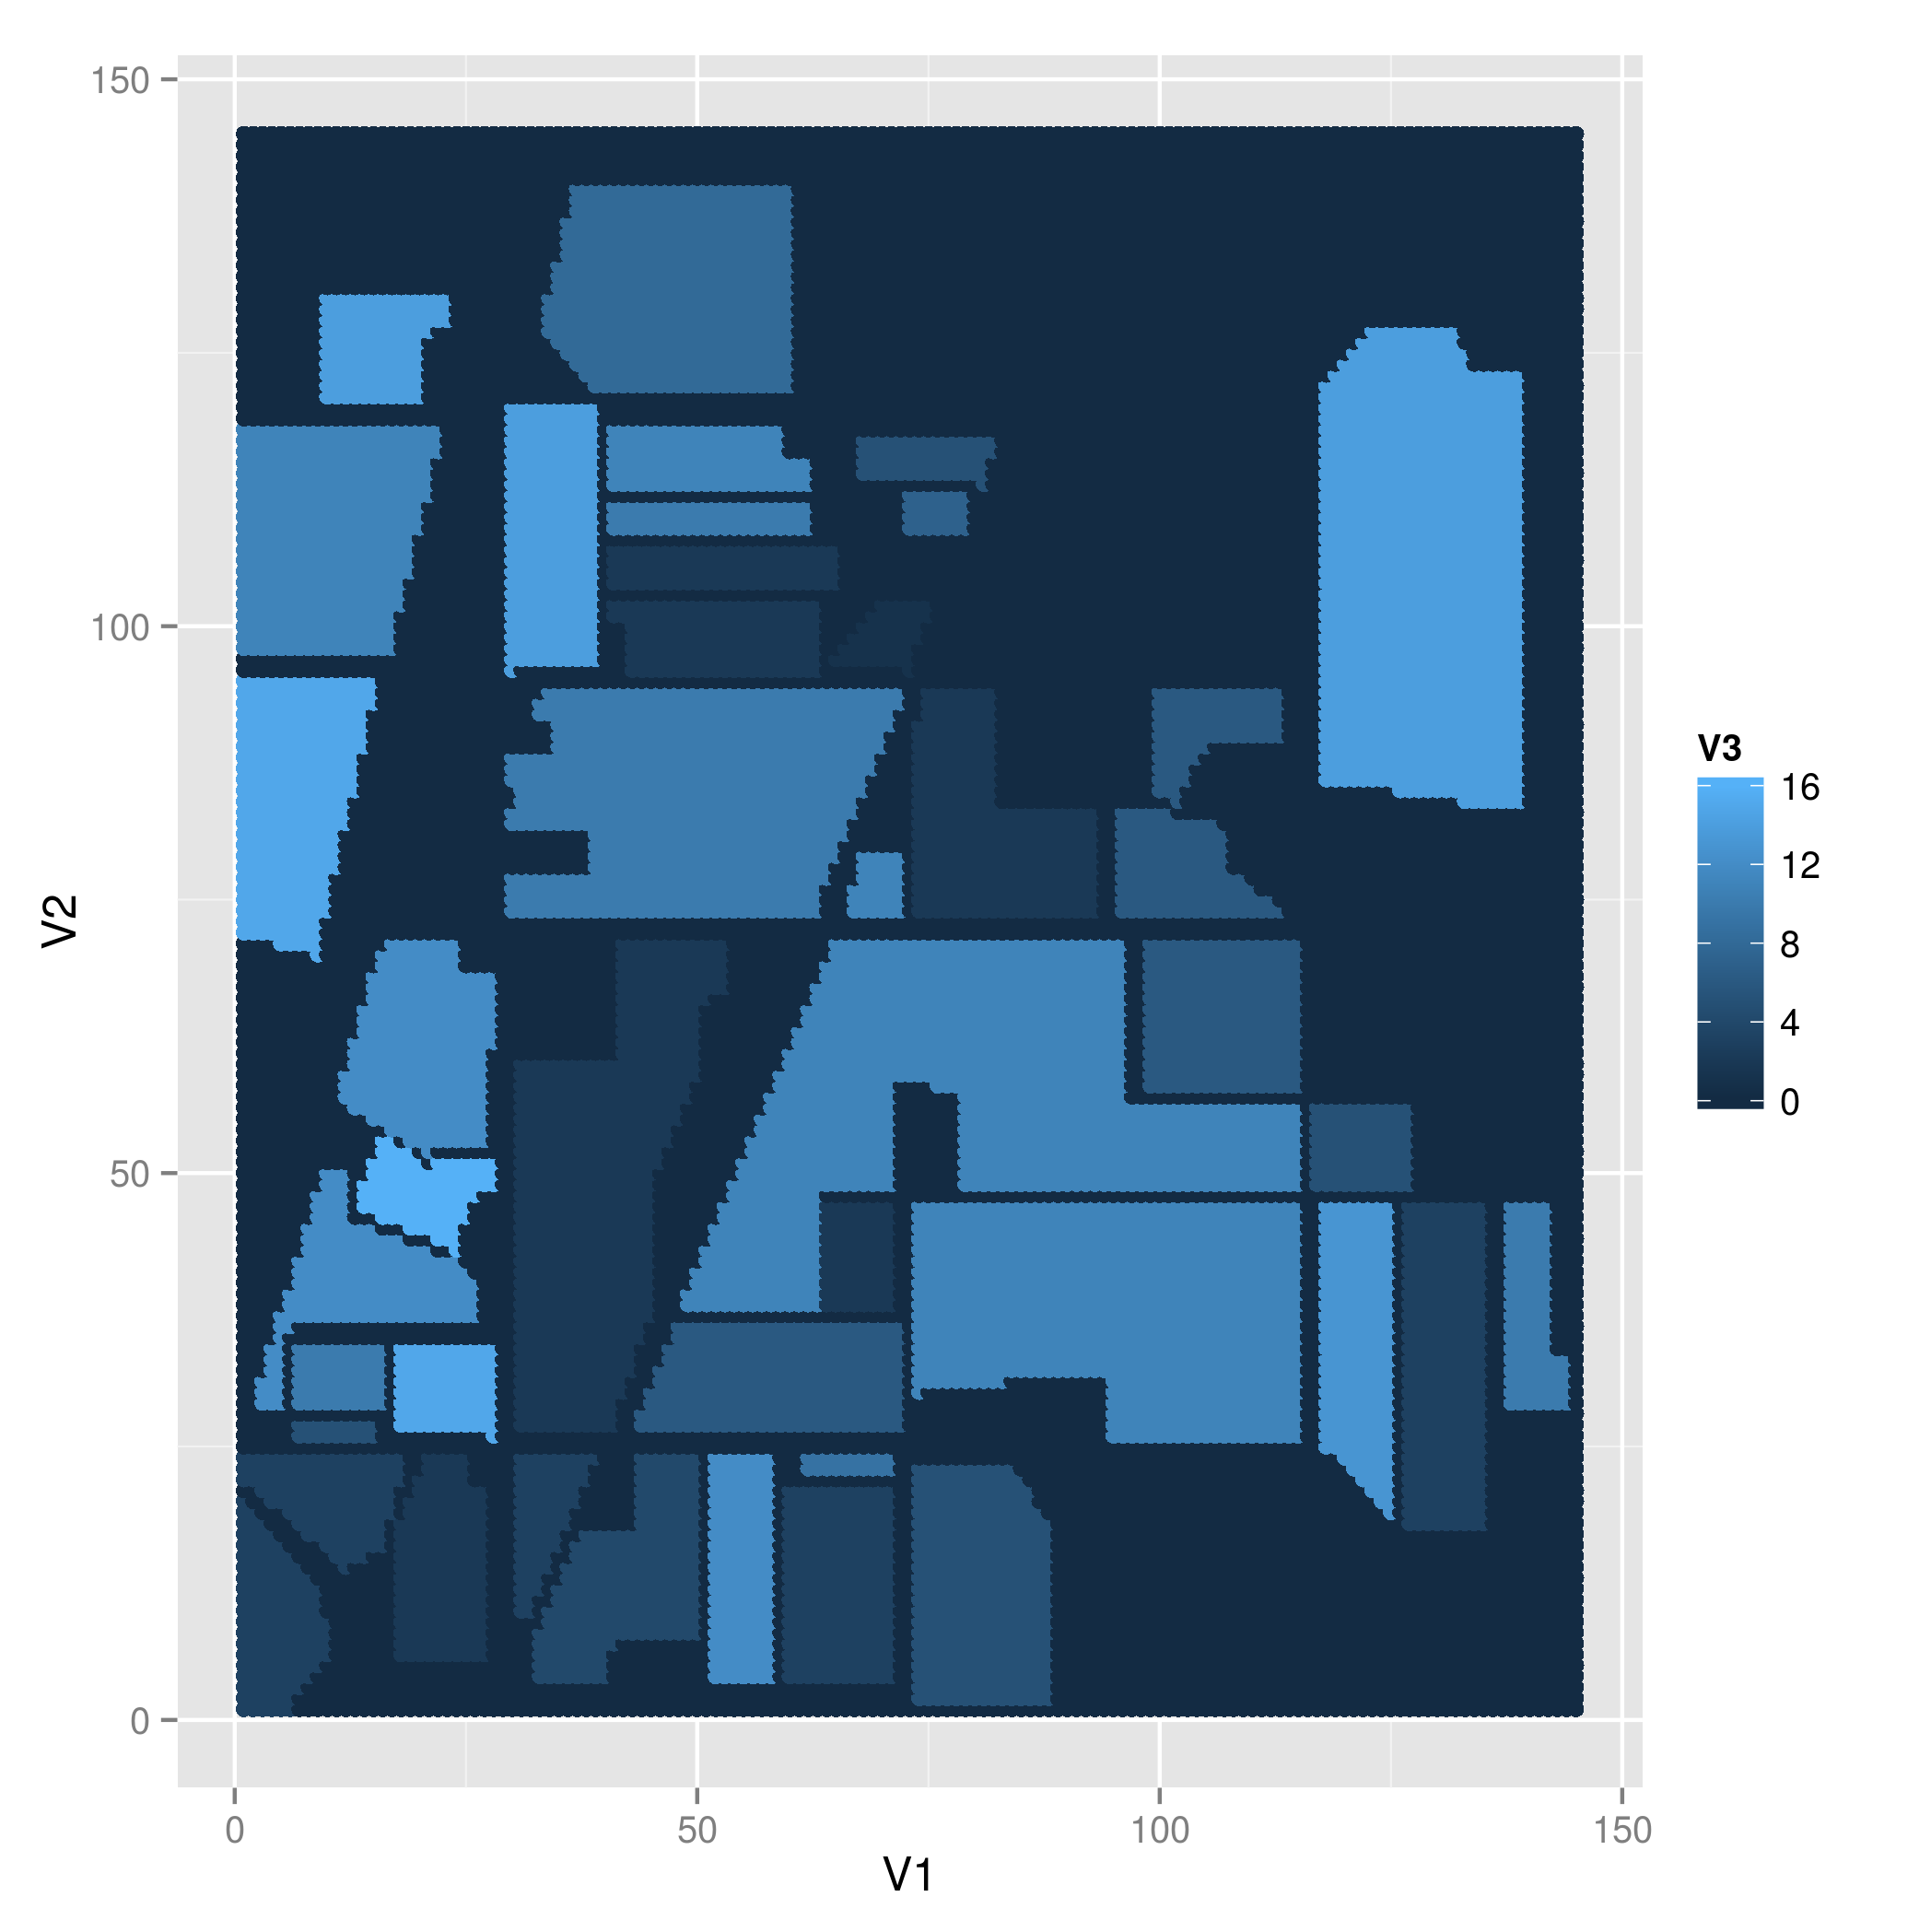
\includegraphics[scale=.3]{gt.png}
\end{column}
\end{columns}
\end{frame}

\begin{frame}{K-Means}
K-Means using 5 classes
\begin{columns}[T]
\begin{column}{.48\textwidth}
% LEFT COLUMN
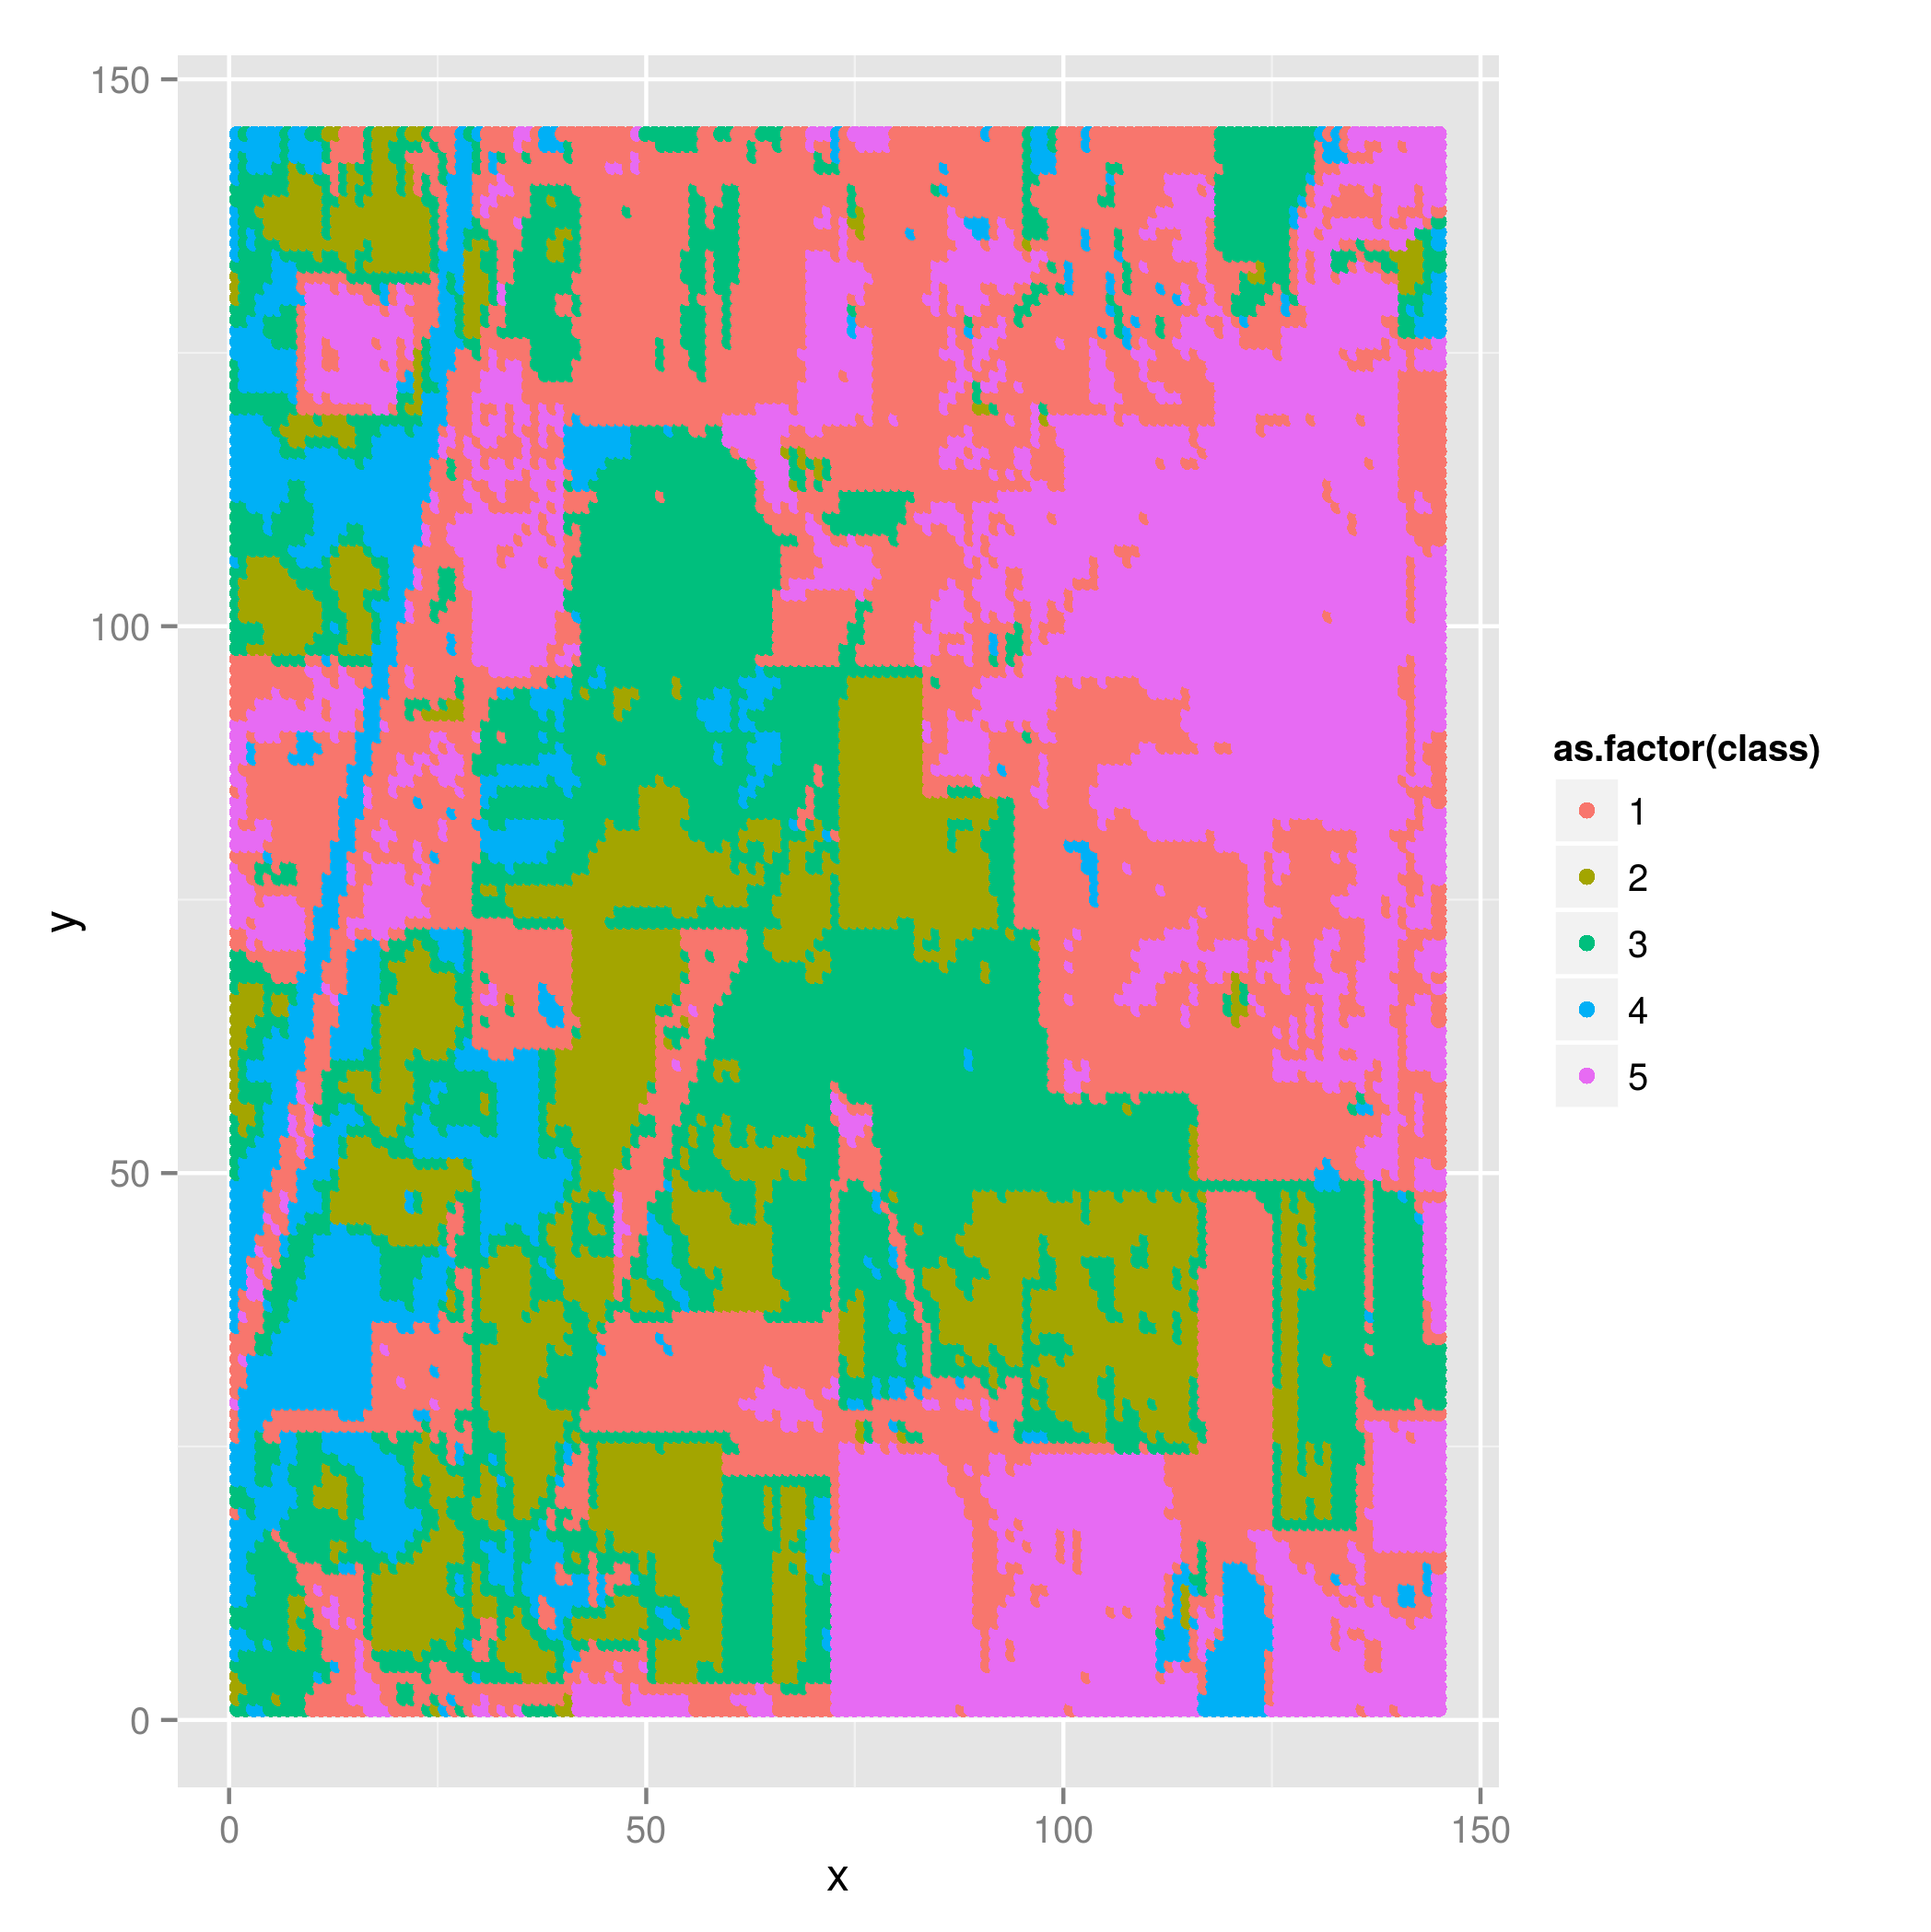
\includegraphics[scale=.3]{km5.png}
\end{column}
\hfill
\begin{column}{.48\textwidth}
% RIGHT COLUMN
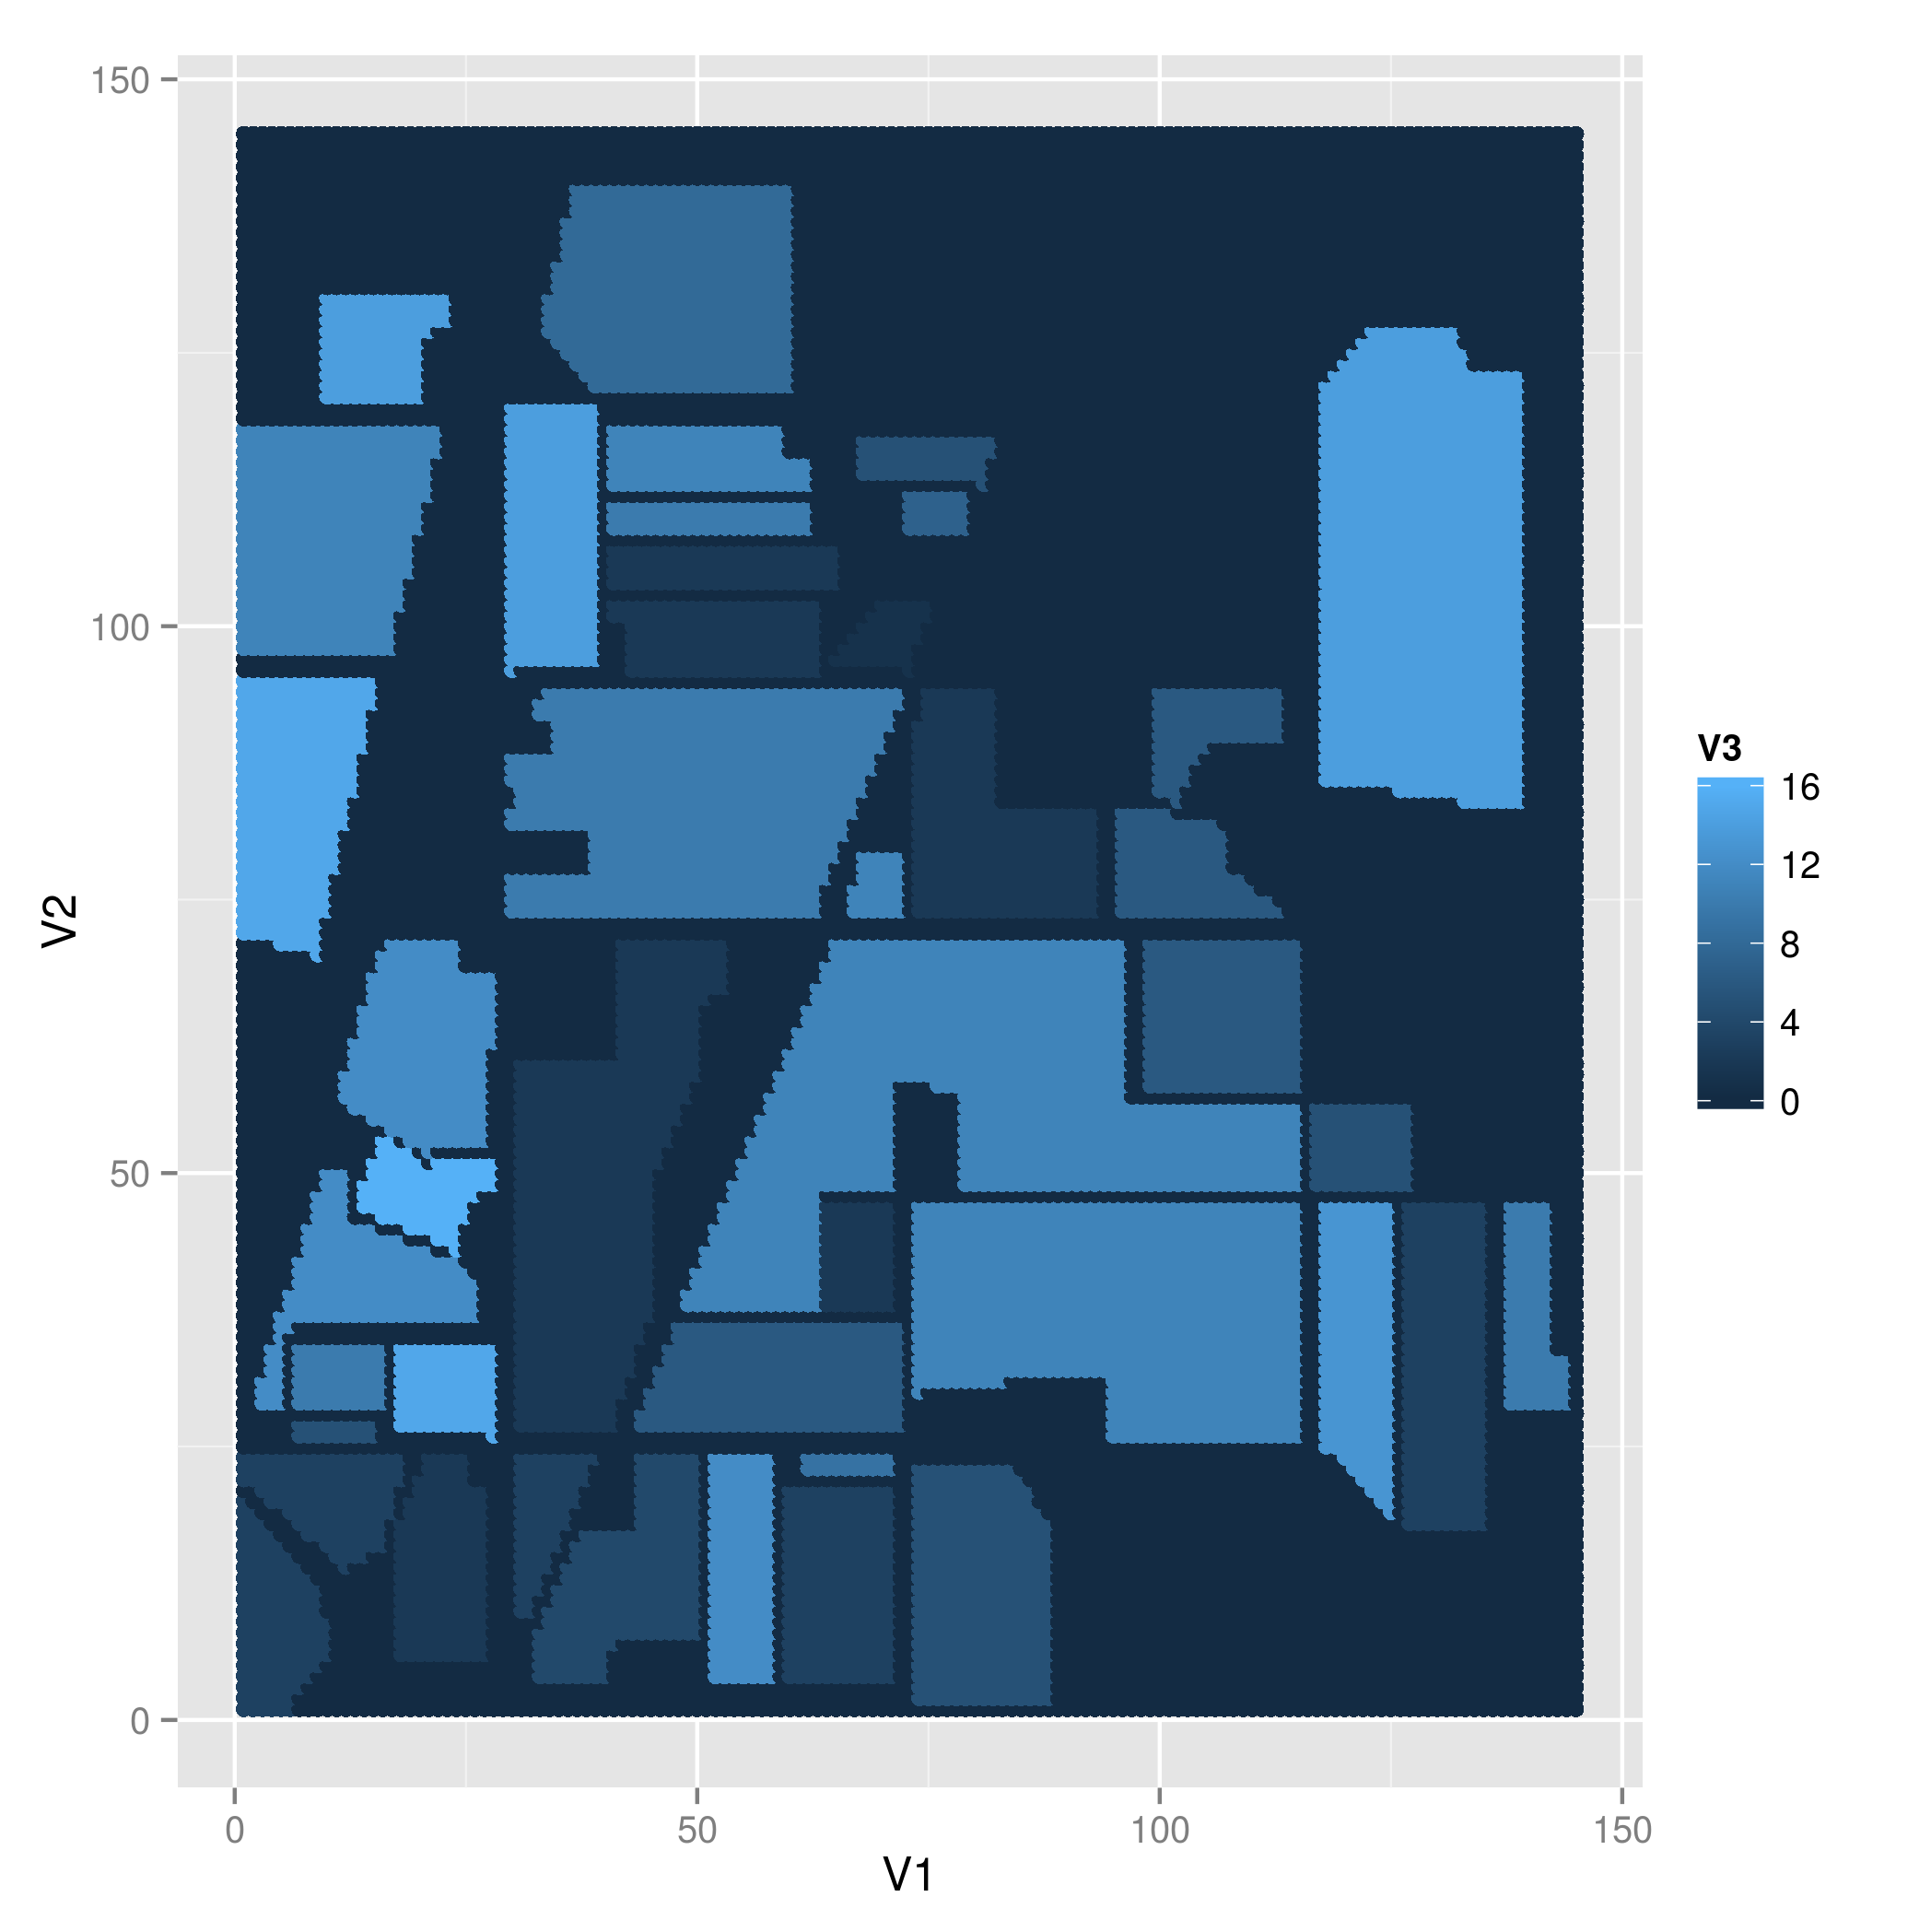
\includegraphics[scale=.3]{gt.png}
\end{column}
\end{columns}
\end{frame}

\subsection{Higher order K-Means}
\begin{frame}{K-Means}
K-Means using 10 classes
\begin{columns}[T]
\begin{column}{.48\textwidth}
% LEFT COLUMN
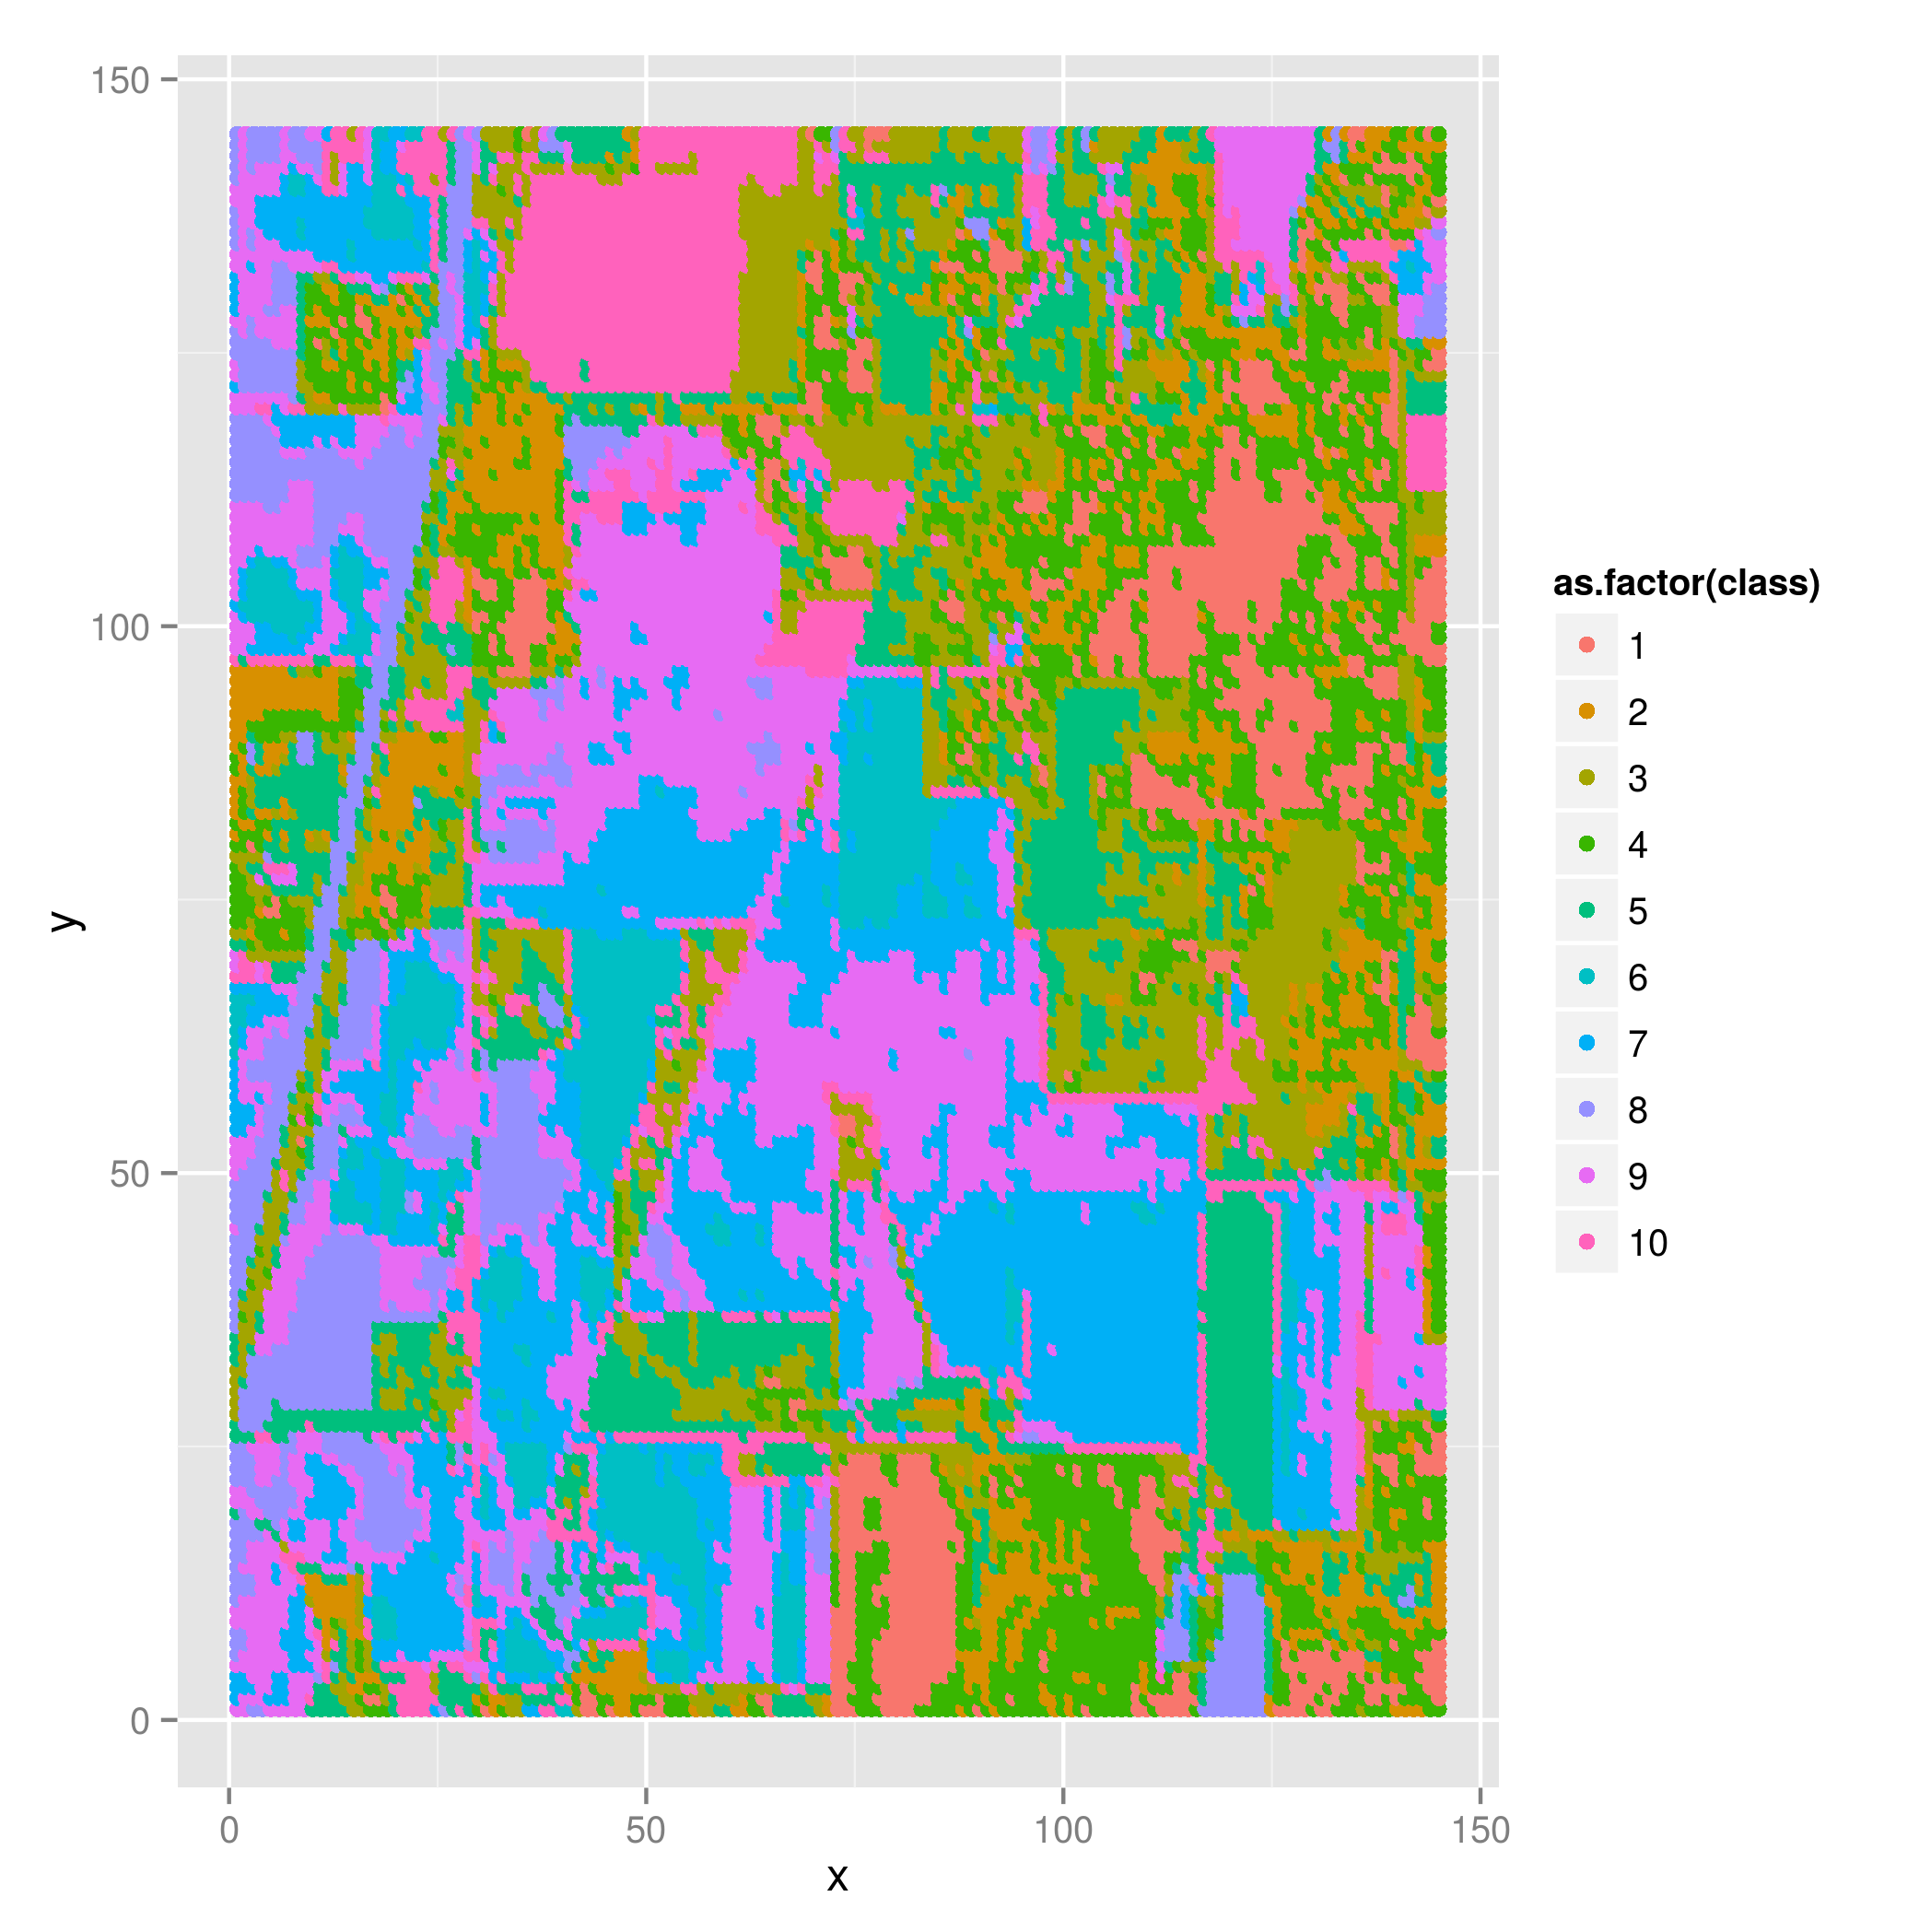
\includegraphics[scale=.3]{km10.png}
\end{column}
\hfill
\begin{column}{.48\textwidth}
% RIGHT COLUMN
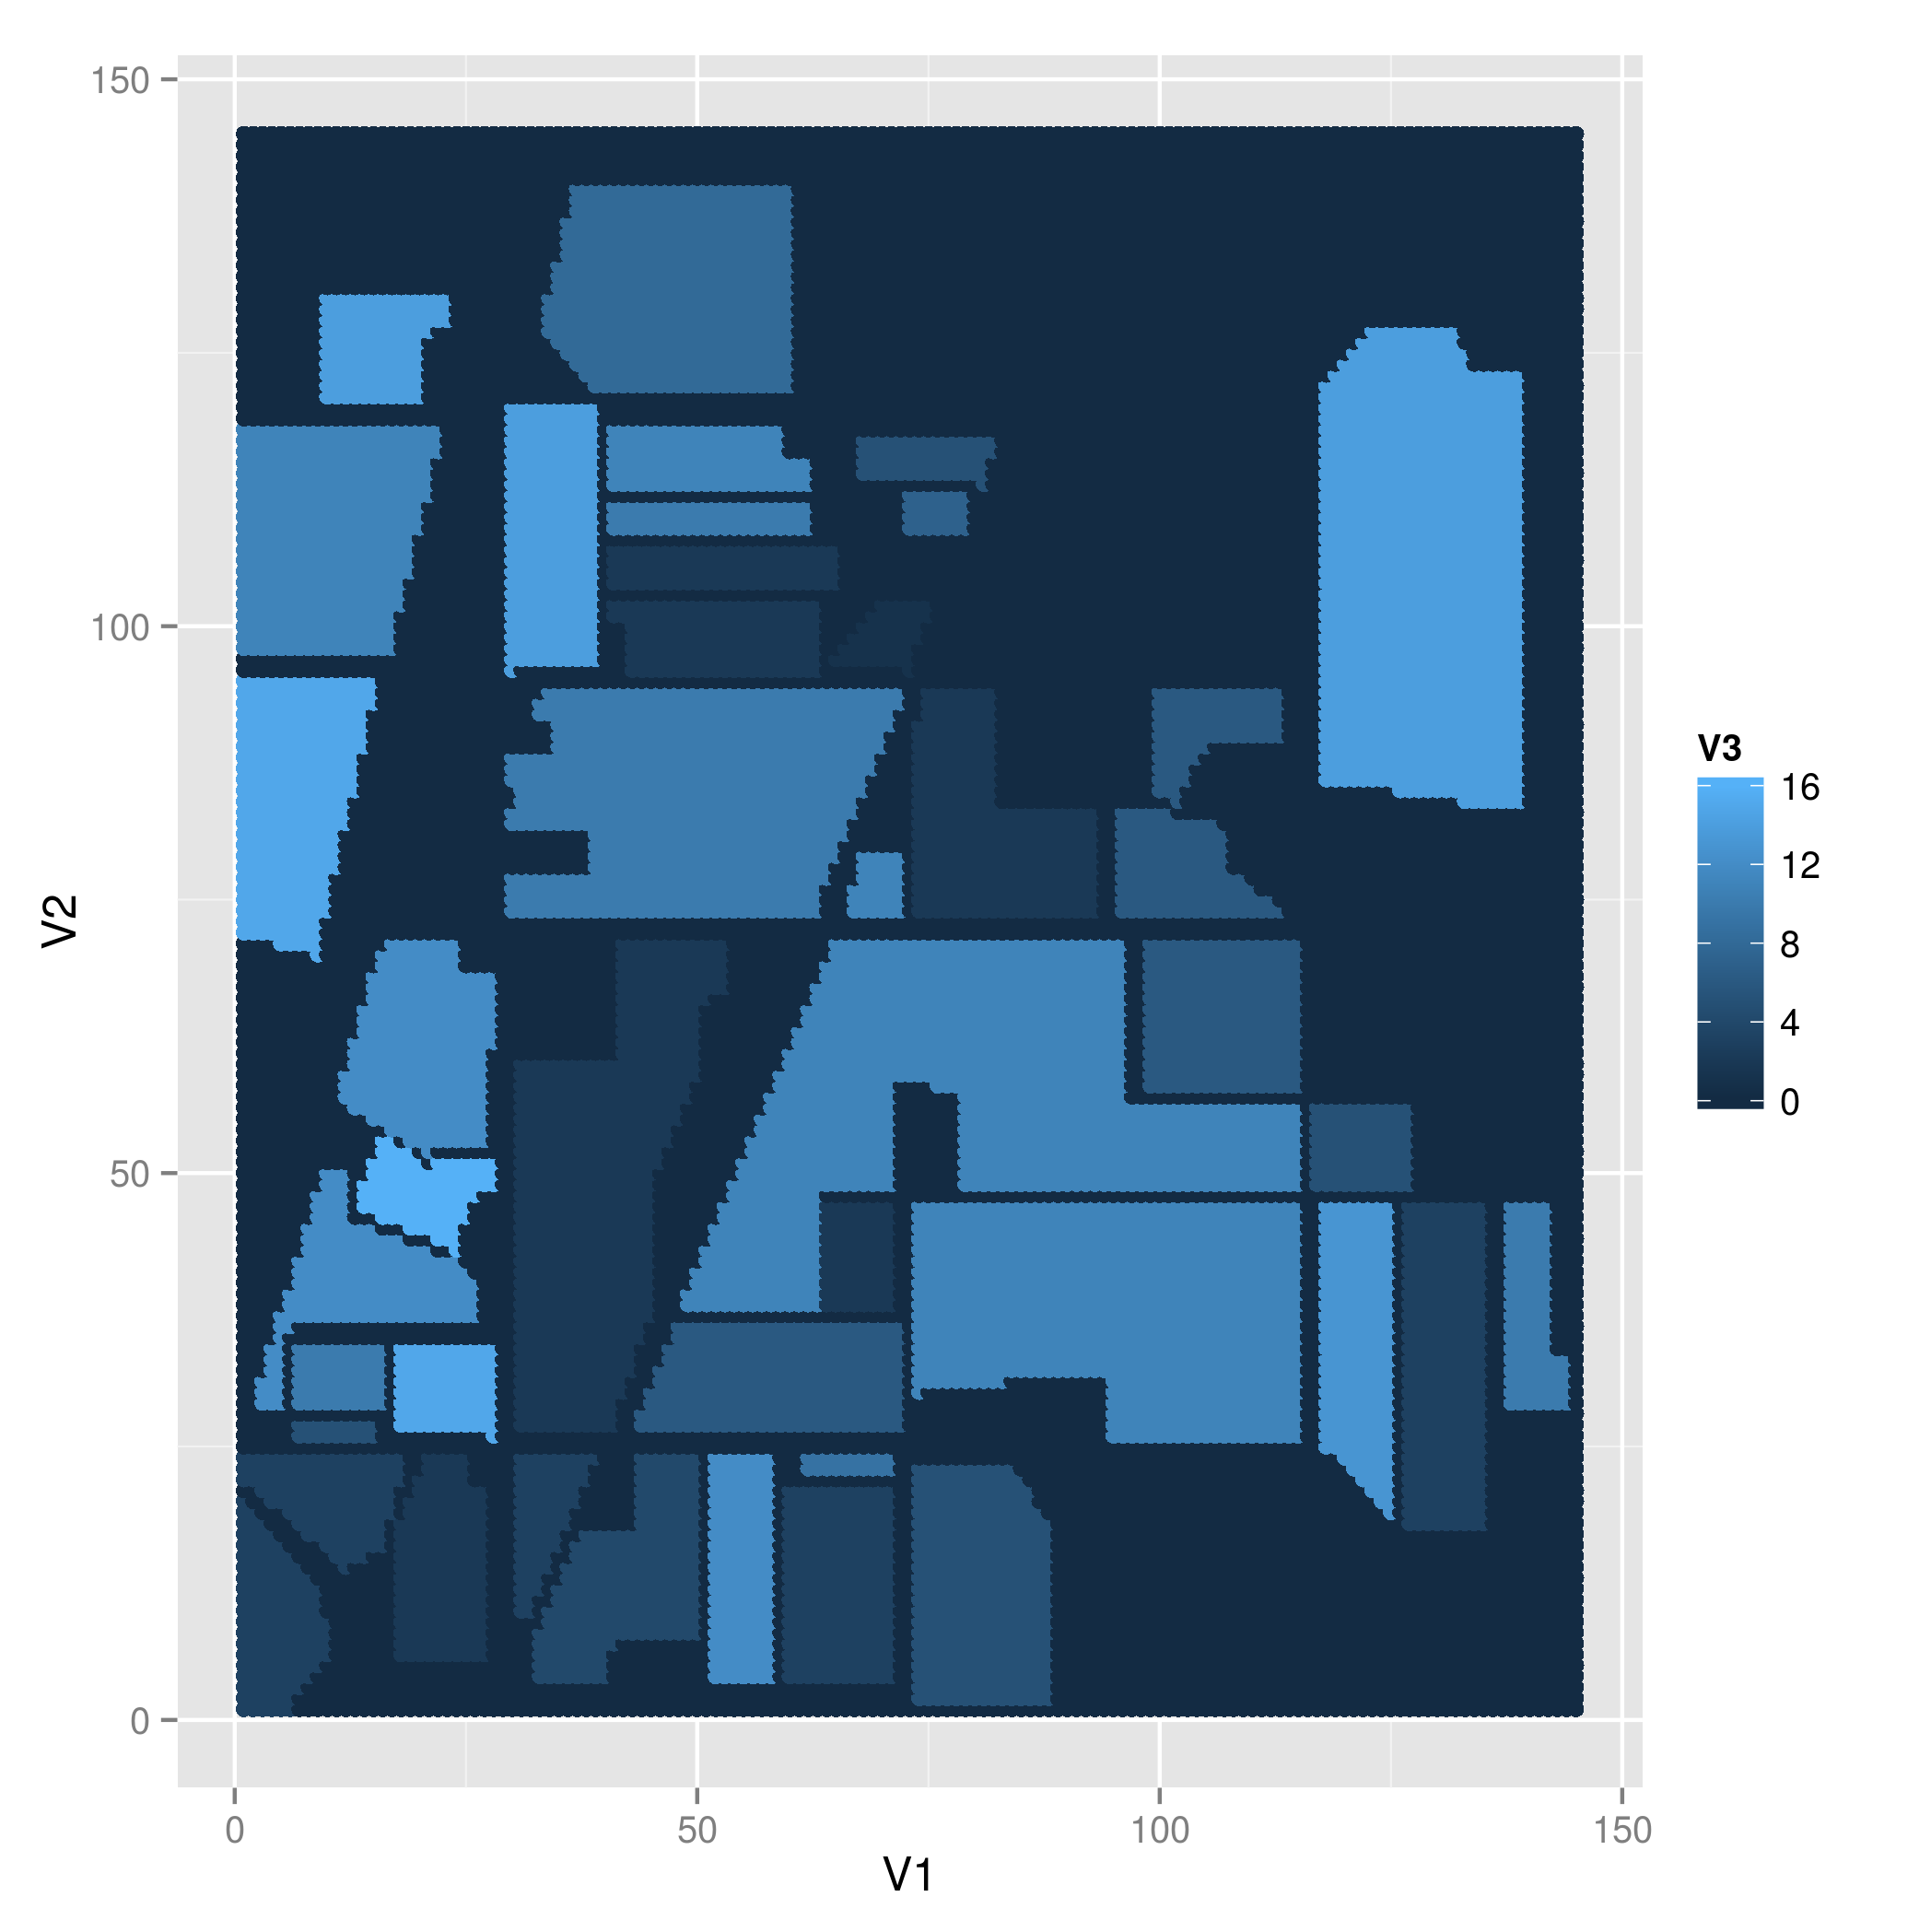
\includegraphics[scale=.3]{gt.png}
\end{column}
\end{columns}
\end{frame}

\begin{frame}{K-Means}
K-Means using 16 classes
\begin{columns}[T]
\begin{column}{.48\textwidth}
% LEFT COLUMN
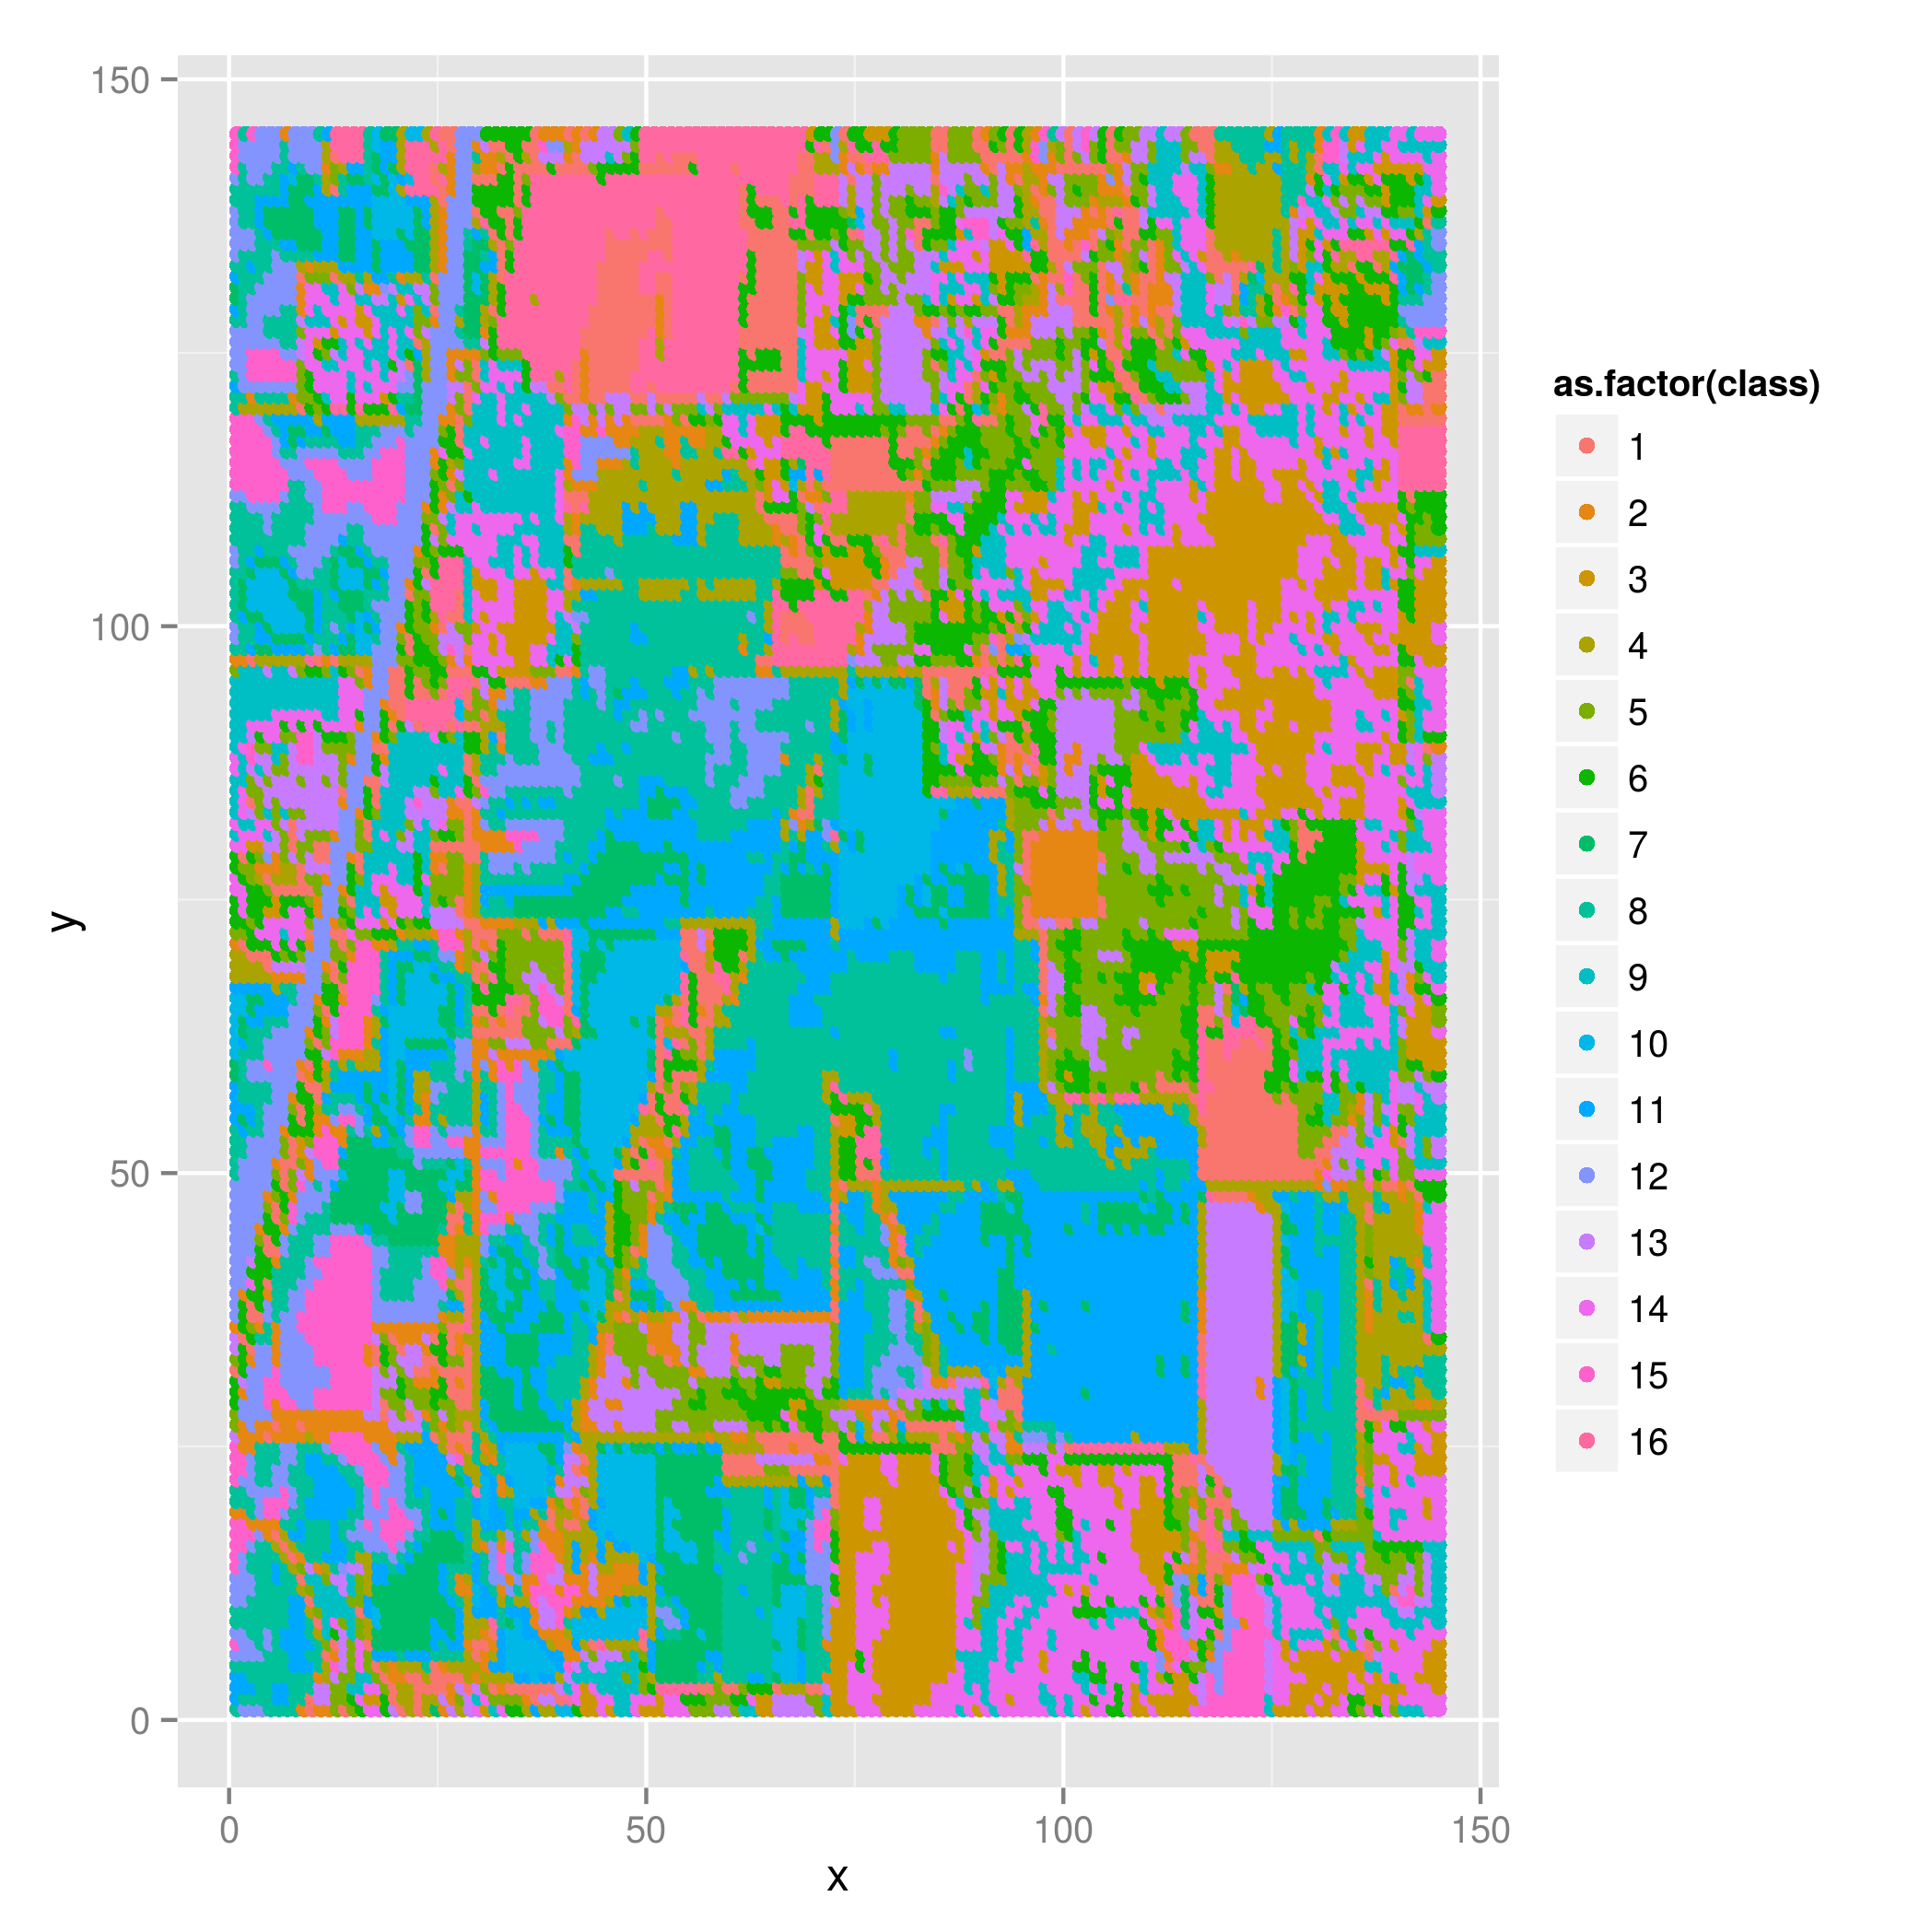
\includegraphics[scale=.3]{km16.png}
\end{column}
\hfill
\begin{column}{.48\textwidth}
% RIGHT COLUMN
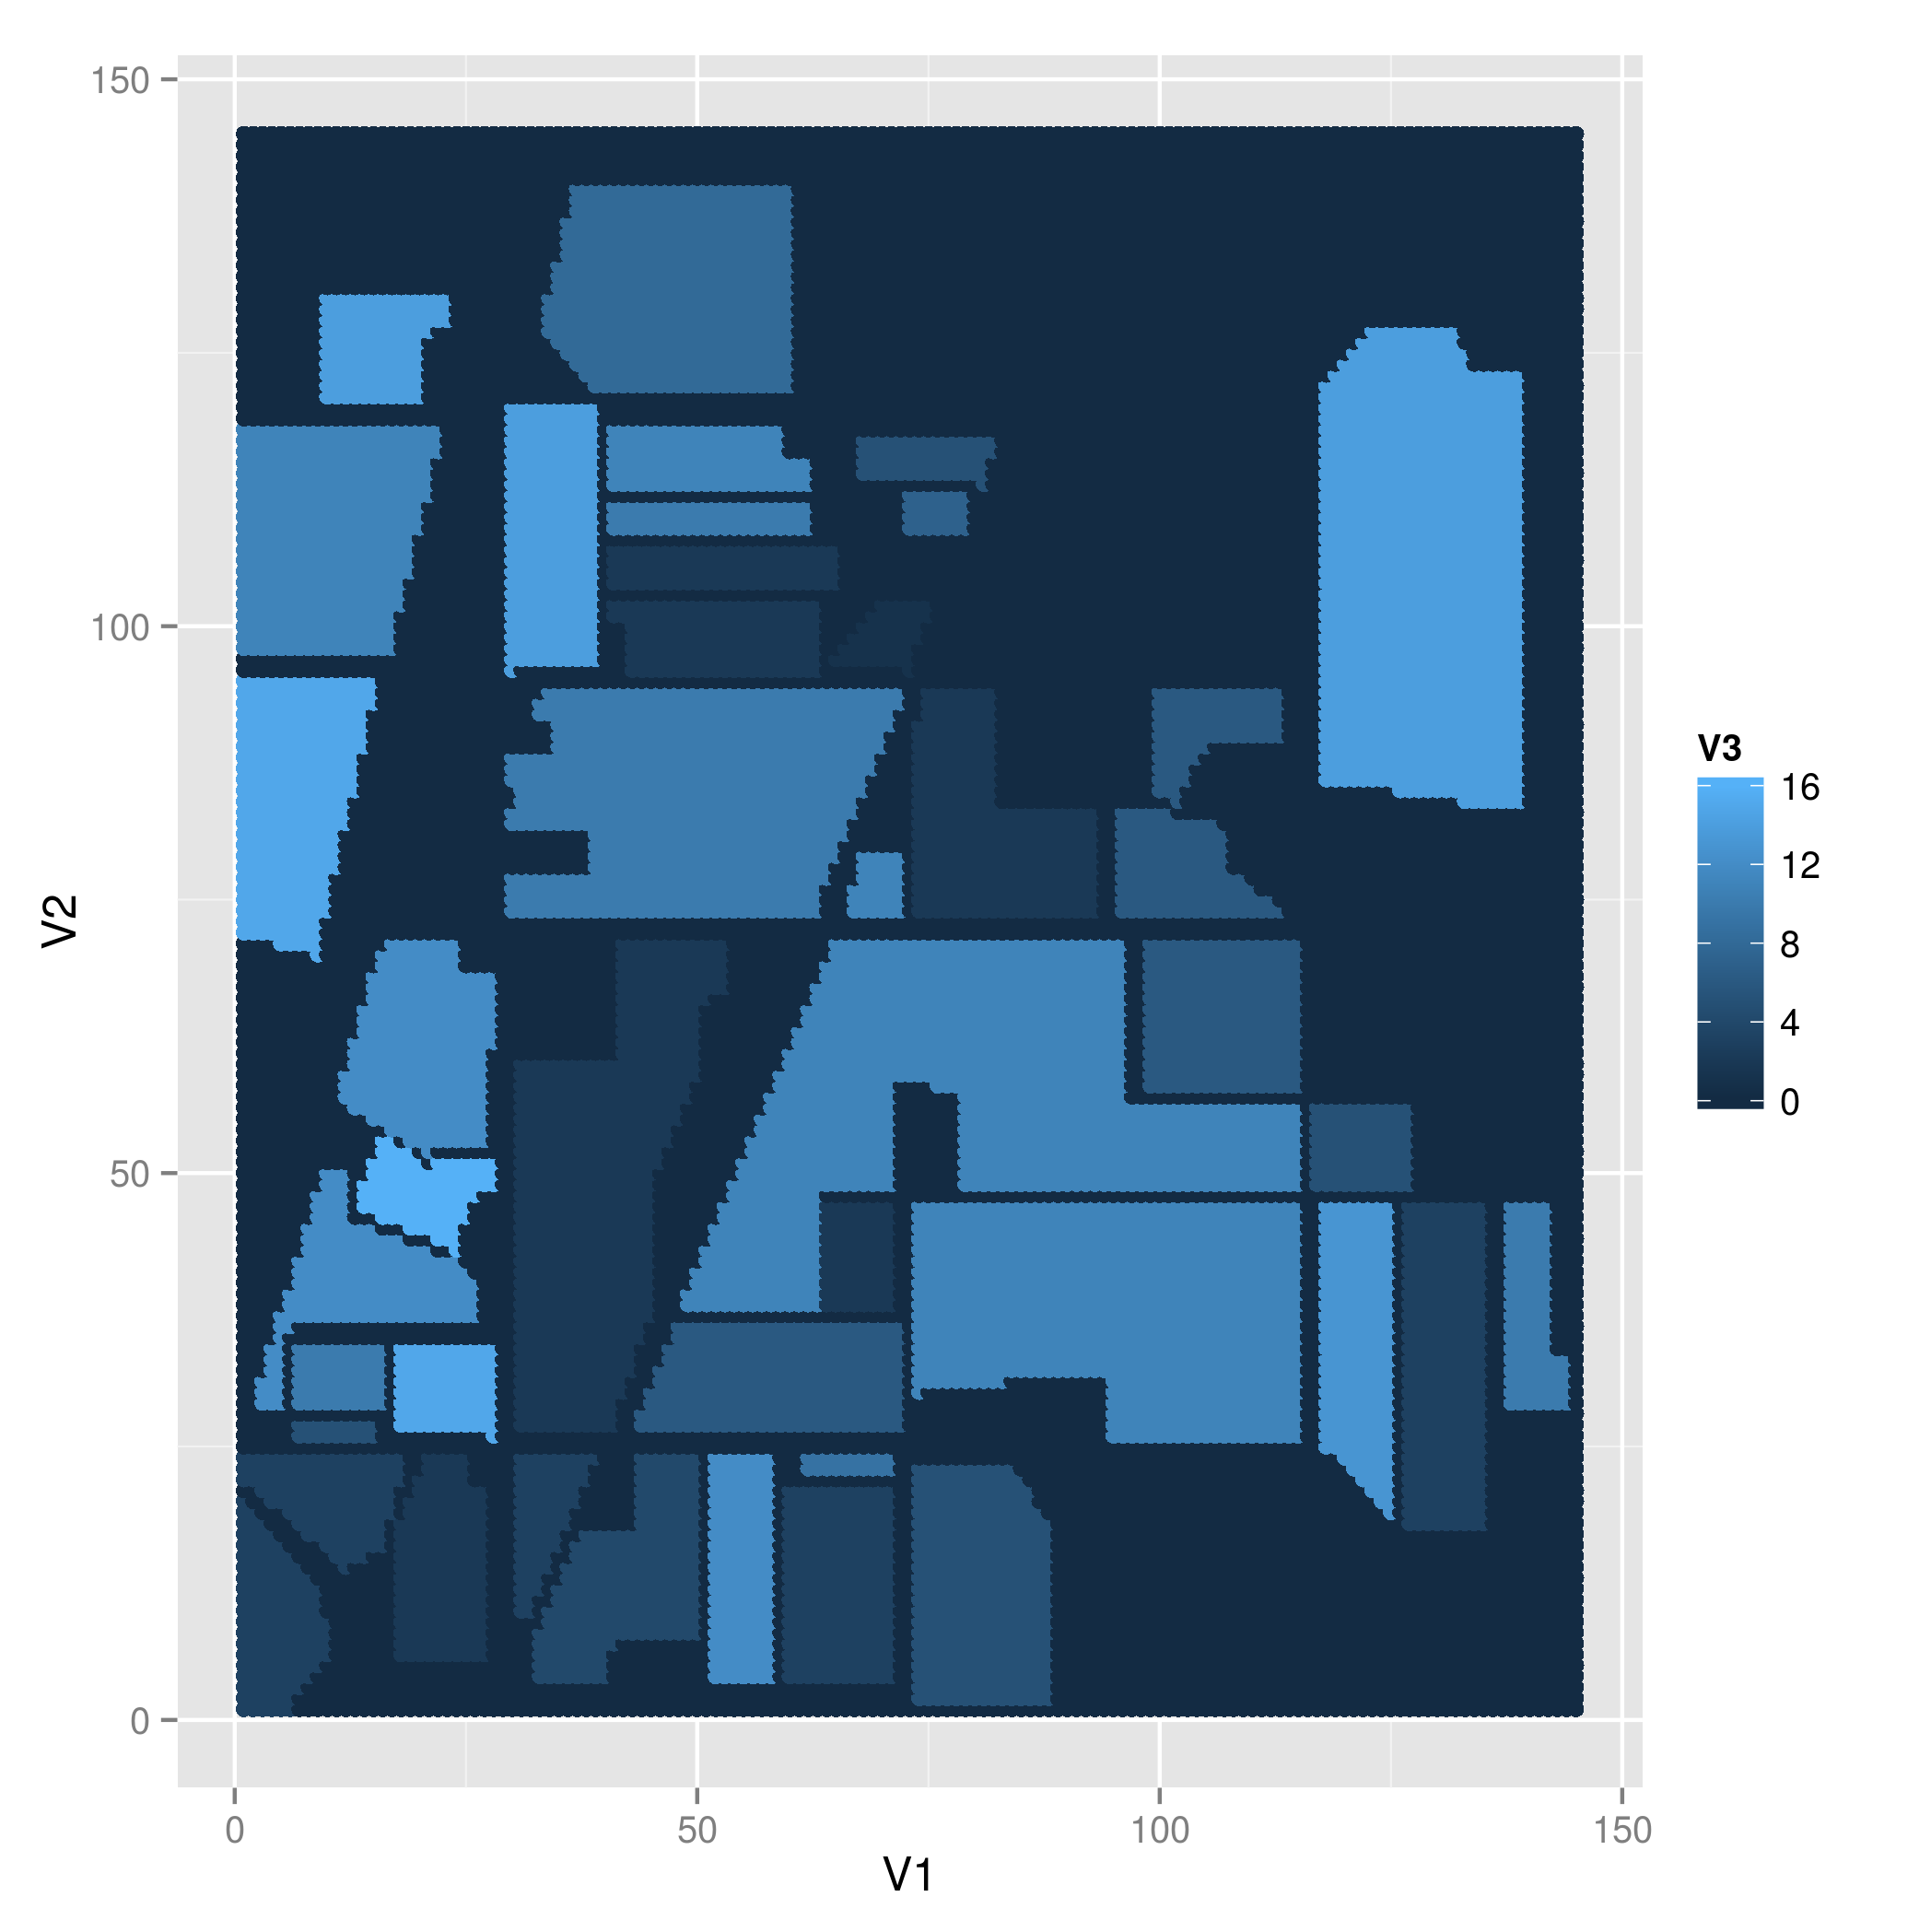
\includegraphics[scale=.3]{gt.png}
\end{column}
\end{columns}
\end{frame}

%%%%%%%%%%%%%%%
%%%   SVM   %%%
%%%%%%%%%%%%%%%

\section{SVM}
\subsection{Soft SVM}
\begin{frame}{Support Vector Machine}
\begin{itemize}
\item Separates data into distinct classes
\item Constructs a hyperplane between classes
\item Soft-margin SVM versus Hard-margin SVM
\end{itemize}
\end{frame}

\begin{frame}{Support Vector Machine}
\begin{columns}[T]
\begin{column}{.48\textwidth}
% LEFT COLUMN
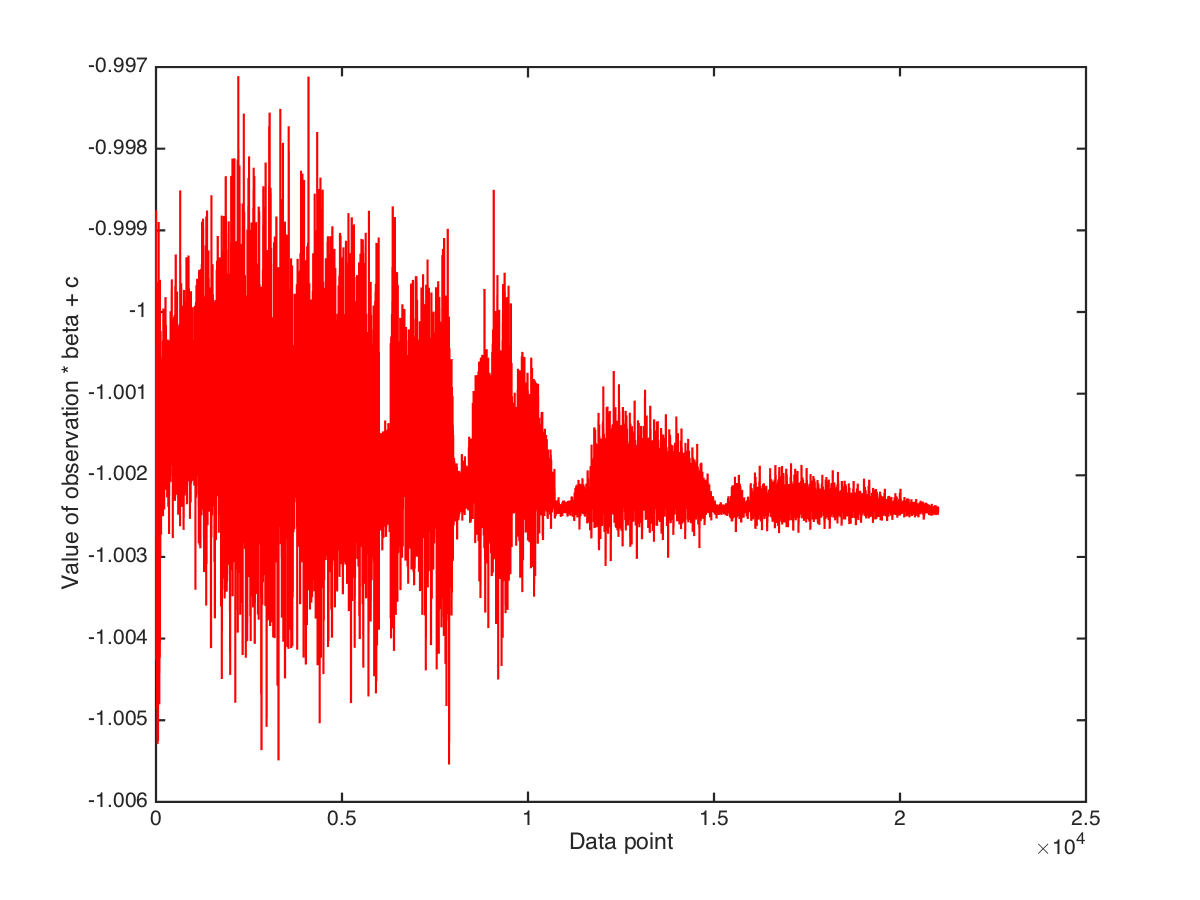
\includegraphics[scale=.3]{softsvmImage.png}
\end{column}
\hfill
\begin{column}{.48\textwidth}
% RIGHT COLUMN
\begin{itemize}
\item Reduced data from 3D to 2D by appending rows (increasing the number of columns)
\item Arbitrarily picked to separate between corn and not corn
\item Soft SVM because of possibility of nonlinear separability and less influence by noise
\end{itemize}
\end{column}
\end{columns}
\end{frame}

%%%%%%%%%%%%%%%%%%%%%%
%%%   Conclusion   %%%
%%%%%%%%%%%%%%%%%%%%%%

\section{Conclusion}
\subsection{Results}
\begin{frame}{Results}
\begin{columns}[T]
\begin{column}{.48\textwidth}
% LEFT COLUMN
\begin{itemize}
\item We started to see land divisions in K-Means
\item A soft SVM would very likely classify better
\item K-Means: increase in the number of classes increases the noise level
\item Soft-Margin SVM: data cannot be separated linearly. Multiclass SVM would provide better results 
\end{itemize}
\end{column}
\hfill
\begin{column}{.48\textwidth}
% RIGHT COLUMN
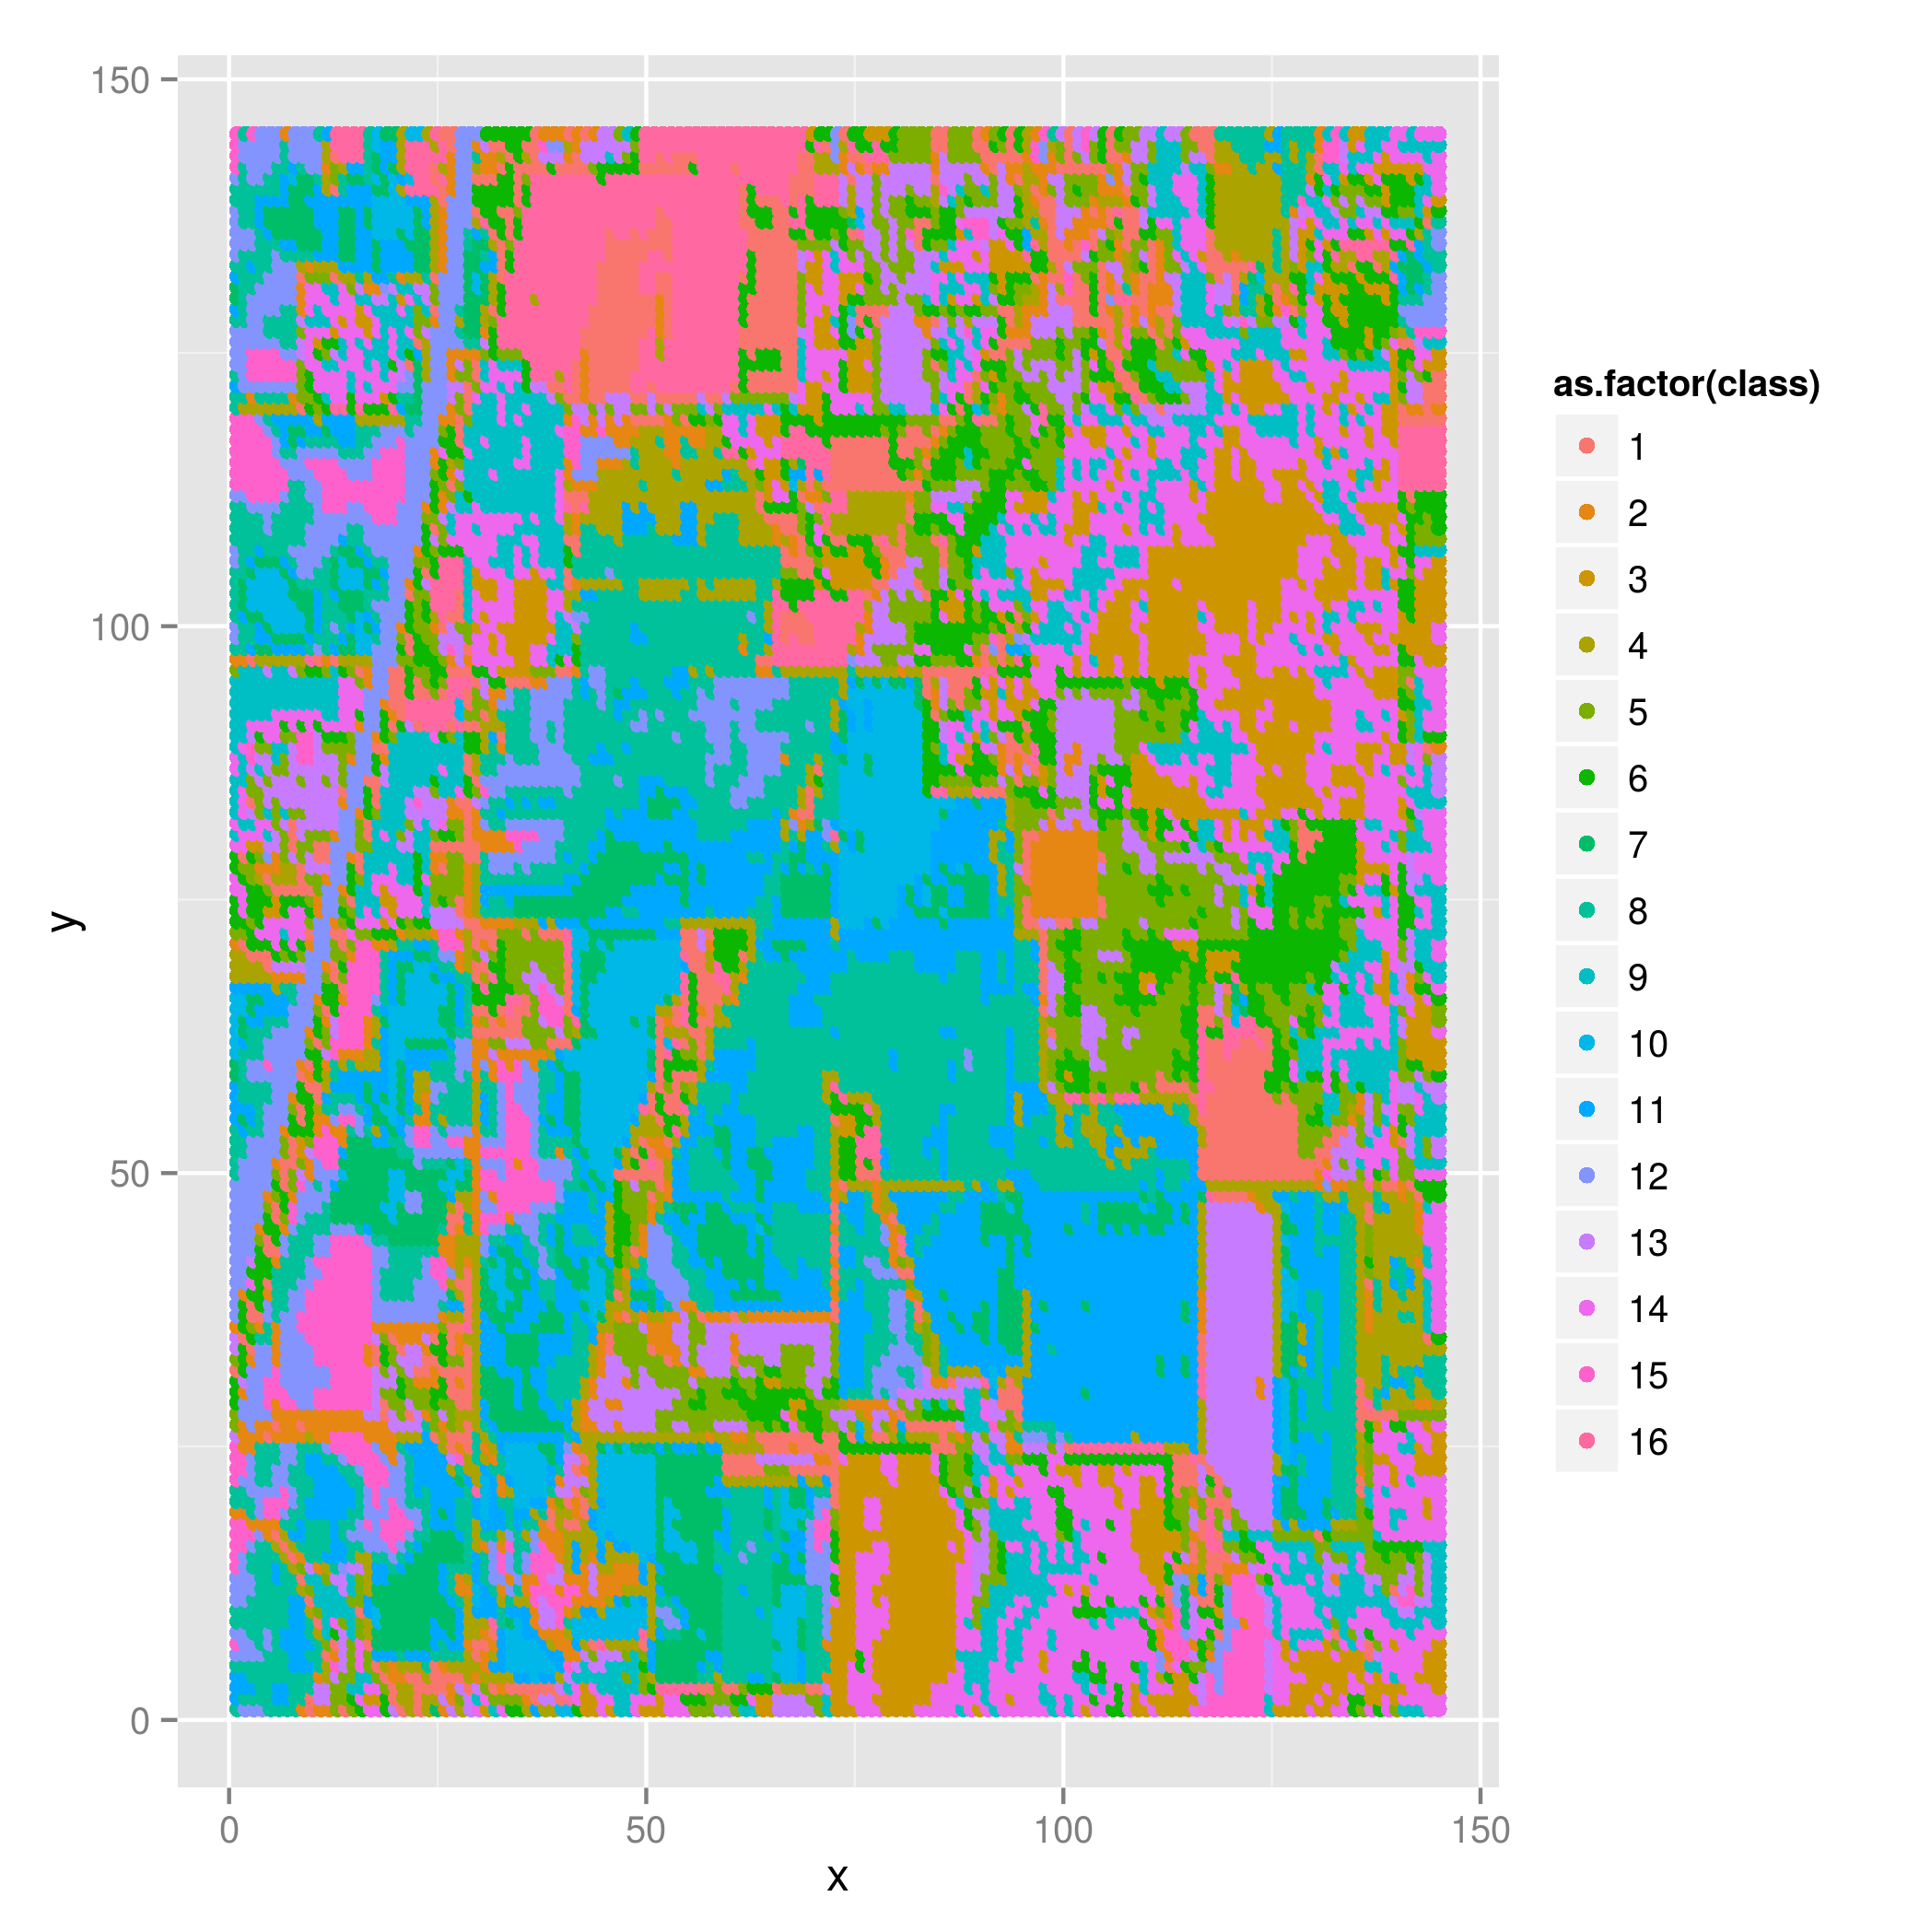
\includegraphics[scale=.3]{km16.png}
\end{column}
\end{columns}
\end{frame}

%%%%%%%%%%%%%%%%%%%%%%%%%%%
%%%   Future Analysis   %%%
%%%%%%%%%%%%%%%%%%%%%%%%%%%

\section{Further Analysis}
\subsection{Noise Detection}
\begin{frame}{Future Ideas}
\begin{columns}[T]
\begin{column}{.48\textwidth}
% LEFT COLUMN
\includegraphics[scale=.35]{wavelength1.png}
\end{column}
\hfill
\begin{column}{.48\textwidth}
% RIGHT COLUMN
\begin{itemize}
\item Some of the data appears noisy
\item This could negatively impact classification
\item Detecting noise and biasing the model towards ``clean'' data could help the prediction
\end{itemize}
\end{column}
\end{columns}
\end{frame}

\subsection{Multiclass Support Vector Machine}
\begin{frame}{Future Ideas}
\begin{columns}[T]
\begin{column}{.48\textwidth}
% LEFT COLUMN
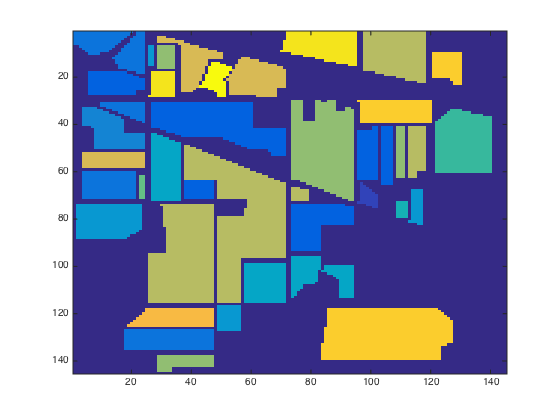
\includegraphics[scale=.35]{groundtruth.png}
\end{column}
\hfill
\begin{column}{.48\textwidth}
% RIGHT COLUMN
\begin{itemize}
\item Implement a multiclass SVM function
\item Completely split the data into 16 classes instead of 2
\item Increase accuracy of data separation
\end{itemize}
\end{column}
\end{columns}
\end{frame}

\end{document}
